%%%%%%%%%%%%%%%%%%%%%%%%%%%%%%%%%%%%%%%%%%%%%%%%%%%%%%%%%%%%%%%%%%%%%
%%                                                                 %%
%% Please do not use \input{...} to include other tex files.       %%
%% Submit your LaTeX manuscript as one .tex document.              %%
%%                                                                 %%
%% All additional figures and files should be attached             %%
%% separately and not embedded in the \TeX\ document itself.       %%
%%                                                                 %%
%%%%%%%%%%%%%%%%%%%%%%%%%%%%%%%%%%%%%%%%%%%%%%%%%%%%%%%%%%%%%%%%%%%%%

%%\documentclass[referee,sn-basic]{sn-jnl}% referee option is meant for double line spacing

%%=======================================================%%
%% to print line numbers in the margin use lineno option %%
%%=======================================================%%

%%\documentclass[lineno,sn-basic]{sn-jnl}% Basic Springer Nature Reference Style/Chemistry Reference Style

%%======================================================%%
%% to compile with pdflatex/xelatex use pdflatex option %%
%%======================================================%%

%%\documentclass[pdflatex,sn-basic]{sn-jnl}% Basic Springer Nature Reference Style/Chemistry Reference Style

%%\documentclass[sn-basic]{sn-jnl}% Basic Springer Nature Reference Style/Chemistry Reference Style

\documentclass[sn-mathphys]{sn-jnl}% Math and Physical Sciences Reference Style

%%\documentclass[sn-aps]{sn-jnl}% American Physical Society (APS) Reference Style
%%\documentclass[sn-vancouver]{sn-jnl}% Vancouver Reference Style
%%\documentclass[sn-apa]{sn-jnl}% APA Reference Style
%%\documentclass[sn-chicago]{sn-jnl}% Chicago-based Humanities Reference Style
%%\documentclass[sn-standardnature]{sn-jnl}% Standard Nature Portfolio Reference Style
%%\documentclass[default]{sn-jnl}% Default
%%\documentclass[default,iicol]{sn-jnl}% Default with double column layout

%%%% Standard Packages
%%<additional latex packages if required can be included here>
%%%%

%%%%%=============================================================================%%%%
%%%%  Remarks: This template is provided to aid authors with the preparation
%%%%  of original research articles intended for submission to journals published 
%%%%  by Springer Nature. The guidance has been prepared in partnership with 
%%%%  production teams to conform to Springer Nature technical requirements. 
%%%%  Editorial and presentation requirements differ among journal portfolios and 
%%%%  research disciplines. You may find sections in this template are irrelevant 
%%%%  to your work and are empowered to omit any such section if allowed by the 
%%%%  journal you intend to submit to. The submission guidelines and policies 
%%%%  of the journal take precedence. A detailed User Manual is available in the 
%%%%  template package for technical guidance.
%%%%%=============================================================================%%%%

\jyear{2023}%

%% as per the requirement new theorem styles can be included as shown below
\theoremstyle{thmstyleone}%
\newtheorem{theorem}{Theorem}%  meant for continuous numbers
%%\newtheorem{theorem}{Theorem}[section]% meant for sectionwise numbers
%% optional argument [theorem] produces theorem numbering sequence instead of independent numbers for Proposition
\newtheorem{proposition}[theorem]{Proposition}% 
%%\newtheorem{proposition}{Proposition}% to get separate numbers for theorem and proposition etc.

\theoremstyle{thmstyletwo}%
\newtheorem{example}{Example}%
\newtheorem{remark}{Remark}%

\theoremstyle{thmstylethree}%
\newtheorem{definition}{Definition}%
\usepackage{amsmath}
\usepackage{subfig}

\raggedbottom
%%\unnumbered% uncomment this for unnumbered level heads

\begin{document}

\title[Physics Constrained Deep Learning for Ptychographic Reconstruction]{Physics Constrained Unsupervised Deep Learning for Rapid, High Resolution Scanning Coherent Diffraction Reconstruction}

%%=============================================================%%
%% Prefix	-> \pfx{Dr}
%% GivenName	-> \fnm{Joergen W.}
%% Particle	-> \spfx{van der} -> surname prefix
%% FamilyName	-> \sur{Ploeg}
%% Suffix	-> \sfx{IV}
%% NatureName	-> \tanm{Poet Laureate} -> Title after name
%% Degrees	-> \dgr{MSc, PhD}
%% \author*[1,2]{\pfx{Dr} \fnm{Joergen W.} \spfx{van der} \sur{Ploeg} \sfx{IV} \tanm{Poet Laureate} 
%%                 \dgr{MSc, PhD}}\email{iauthor@gmail.com}
%%=============================================================%%

\author*[1,2]{\fnm{First} \sur{Author}}\email{iauthor@gmail.com}

\author[2,3]{\fnm{Second} \sur{Author}}\email{iiauthor@gmail.com}

\author[1,2]{\fnm{Third} \sur{Author}}\email{iiiauthor@gmail.com}

\affil*[1]{\orgdiv{Department}, \orgname{Organization}, \orgaddress{\street{Street}, \city{City}, \postcode{100190}, \state{State}, \country{Country}}}

% \affil[2]{\orgdiv{Department}, \orgname{Organization}, \orgaddress{\street{Street}, \city{City}, \postcode{10587}, \state{State}, \country{Country}}}



%%==================================%%
%% sample for unstructured abstract %%
%%==================================%%

%\abstract{The phase problem of coherent diffractive imaging (CDI) is fundamental to lensless imaging in an array of scientific fields, ranging from X ray science to astronomy. Existing techniques for solving the phase problem rely on algorithms that are iterative and -- consequently -- slow, which greatly hampers their use in synchrotron and XFEL environments. Deep learning based approaches demonstrate impressive speedups at the expense of imaging quality and an onerous need for large amounts of labeled training data, but recent progress has largely solved these two weaknesses through \emph{unsupervised} deep learning (DL) methods that incorporate diffraction physics within the model (physics-informed neural networks: PINNs). In this work we introduce a new reconstruction approach using a representative CDI technique, ptychography. We extend the PINN concept by combining the diffraction forward map with a second physics-based constraint based on measurement overlaps. We also consider the previously-neglected effects of shot noise in the diffraction measurement and find that a corresponding negative log likelihood loss function, evaluated over the predictive pdf of photon counts, yields a much more robust model than conventional choices such as MAE or MSE. Our resulting approach, PtychoPINN, retains the intrinsic speed of DL-based reconstruction (1000-fold that of iterative solvers) while greatly improving upon the accuracy, resolution, and generalizability of prior state-of-the-art DL-based ptychographic reconstruction, with 3- to 10-fold reductions in reconstruction error.  }

\abstract{The phase problem of coherent diffractive imaging (CDI) is fundamental to lensless imaging in an array of scientific fields, ranging from X ray science to astronomy. Existing techniques for solving the phase problem rely on algorithms that are iterative and -- consequently -- slow, which greatly hampers their use in synchrotron and XFEL environments. Deep learning based approaches demonstrate impressive speedups at the expense of imaging quality and an onerous need for large amounts of labeled training data, but recent progress has largely solved these two weaknesses through \emph{unsupervised} deep learning (DL) methods that incorporate diffraction physics within the model (physics-informed neural networks: PINNs). In this work we introduce a new reconstruction approach using a representative CDI technique, ptychography. We extend the PINN concept by combining the diffraction forward map with a second physics-based constraint based on measurement overlaps. Our resulting approach, PtychoPINN, retains the intrinsic speed of DL-based reconstruction (1000-fold that of iterative solvers) while greatly improving upon the accuracy, resolution, and generalizability of prior state-of-the-art DL-based ptychographic reconstruction, with 5- to 10-fold improvements in spatial resolution.}

%  for bandwidth-limited real-space objects that are close-ish to bandwidth-limited

% conclusion: mention the aleatoric uncertainty there, no need to have in the abstract
% bunch together 2.4 and 3, call it 'results and discussion'
% publish in scientific reports? bring up the fee at next meeting.

% see that ptychoNN is dominated by scaled phase (relative error)
% v vs. inverted v
% absolute value of phase is ill defined, 

%%================================%%
%% Sample for structured abstract %%
%%================================%%



%\keywords{keyword1, Keyword2, Keyword3, Keyword4}

%%\pacs[JEL Classification]{D8, H51}

%%\pacs[MSC Classification]{35A01, 65L10, 65L12, 65L20, 65L70}

\maketitle

%\cite{epie}

% text version of the introduction, v2
\section{Introduction }\label{sec1}
Phase retrieval is a crucial problem in various instances of coherent diffractive imaging (CDI), including nanoscale imaging techniques such as Bragg coherent diffractive imaging reconstruction (BCDI) and ptychography (electron and X-ray), optical super-resolution, and astronomical wavefront sensing. These lensless imaging methods offer unique capabilities by eliminating the limitations of optics, enabling diffraction-limited imaging across a broader range of settings \cite{dean2006phase, heintzmann2021answers, miao2015beyond}. However, in all such configurations, the measured quantity - the number of photons on a detector pixel - depends solely on the amplitude of the diffracted wave. To construct real-space images, the lost phase information must be recovered by solving the inverse problem of phase retrieval, typically done using iterative methods \cite{epie}. Unfortunately, the computational cost of these algorithms hinders CDI in high-throughput or in situ settings, and such methods often suffer from noise sensitivity and convergence issues.

A considerable body of literature focuses on applying deep learning (DL) to inverse problems, with significant success in employing neural networks (NNs) to solve the CDI phase problem much more rapidly than conventional iterative methods \cite{ratner2021recovering,yao2022autophasenn}. Early efforts utilized supervised neural networks to achieve several-orders of magnitude speed improvements, accompanied by two major drawbacks: degradation in reconstruction quality and the need for large volumes of high-quality labeled training data. More recently, strategies such as incorporating the diffraction forward map into deep learning models have been introduced to eliminate the requirement for labels. These models are particularly appealing because they combine unsupervised training with reconstruction quality comparable to (or approaching) that of supervised methods.

Despite the initial success of these models, applications of physics-informed neural networks (PINNs) to CDI have not explored physical priors or constraints beyond the diffraction forward map and discrete Fourier transform (DFT) sampling requirements, nor have they modeled any stochasticity of the relevant physics. \emph{flow} It is conceivable that additional constraints and principled probabilistic treatments could enhance both accuracy and generalization.

In this work, we further develop the PINN computational approach to CDI, specifically for ptychographic reconstruction. We integrate three elements: unsupervised training using the diffraction forward map, additional physics-based constraints informed by the ptychography setup, and an explicitly probabilistic treatment of photon counting (Poisson) statistics. We find that this unique combination of model features merges the advantages of a standard PINN approach, namely speed and unsupervised training, with significantly better reconstruction accuracy than other NN-based solvers, including physics-informed approaches.

%Phase retrieval is a critical problem in several instances of coherent diffractive imaging (CDI), including nanoscale imaging such as Bragg coherent diffractive imaging reconstruction (BCDI) and ptychography (electron and X-ray), optical super-resolution, and astronomical wavefront sensing. These lensless imaging techniques provide a unique capability by eliminating the limitations of optics and allowing diffraction-limited imaging in a wider range of settings \cite{dean2006phase, heintzmann2021answers, miao2015beyond}. However, in all such configurations, the measured quantity - the number of photons on a detector pixel - depends on the amplitude alone of the diffracted wave. To construct real space images, the lost phase information must be recovered by solving the inverse problem of phase retrieval, typically done using iterative methods \cite{epie}. Unfortunately, the computational cost of these algorithms precludes CDI in high-throughput or in situ settings, and such methods often suffer from sensitivity to noise and convergence problems.
%
%There is a considerable literature on applications of deep learning (DL) to inverse problems, and within that community, there has been significant success in using neural networks (NNs) to solve the CDI phase problem much more rapidly than is possible with conventional iterative methods \cite{ratner2021recovering,yao2022autophasenn}. Early efforts used supervised neural networks to extract several-orders of magnitude speedups, with two considerable caveats: degradation in reconstruction quality and a requirement for large amounts of high-quality labeled training data. More recently, strategies such as incorporating the diffraction forward map into deep learning models have been introduced to remove the need for labels. These models are quite attractive because they combine unsupervised training with reconstruction quality comparable to (or approaching) that of supervised methods.
%
%However, despite the initial success of these models, applications of physics-informed neural networks (PINNs) to CDI have not explored physical priors or constraints other than the diffraction forward map and sampling requirements of the discrete Fourier transform (DFT), nor have they modeled any stochasticity of the relevant physics. \emph{flow} It is plausible that additional constraints and principled probabilistic treatments would improve both accuracy and generalization.
%
%In this work, we further develop the PINN computational approach to CDI for the specific problem of ptychographic reconstruction. We combine three elements: unsupervised training using the diffraction forward map, additional physics-based constraints informed by the ptychography setup, and explicitly probabilistic treatment of photon counting (Poisson) statistics. We find that this particular mix of model features combines the advantages of a vanilla PINN approach, namely speed and unsupervised training, with significantly better reconstruction accuracy than other NN-based solvers, including physics-informed approaches.

%largely due to the mismatch between their deterministic assumptions and the intrinsic stochasticity of diffractive measurements.

% TODO rework the next  two paragraphs
% The accuracy of physics-based reconstruction methods derives from their general nature--that is, they invert the physically correct forward map of far field diffraction and can, at least in principle, find the optimal solution for any input (cites and caveats). However, this difficult nonconvex optimization problem requires incremental, iterative solution schemes that are necessarily computationally expensive (cites).  We might also consider the problem's difficulty from the alternate perspective of the optimization algorithm's implementation in a specific physical setting. Iterative reconstruction is physics-aware but oblivious to regularities in the input data -- therefore for each new diffraction signal it must repeat a redundant calculation from scratch, with no benefit from the prior computational work. 

% % TODO passive voice
% NN-based reconstruction methods take a quite opposite approach: no inductive biases or prior knowledge of the diffraction physics is imposed; instead, a large amount of training data is ingested to fit a large function approximator from scratch. Since prediction from a NN involves a mere single forward pass, the reconstruction is intrinsically rapid at inference time. On the other hand, the lack of inductive biases and physical consistency-enforcing constraints causes such models to have quite poor accuracy and generalization with respect to the underlying physics (conversely, they might capture particular regularities in the data quite well). 

\section{Methods, Models \& Tests}
\subsection{Approach}

Physics-based CDI reconstruction methods are accurate because they invert the physically correct forward map of far field diffraction, making them capable of finding the optimal solution for any input, at least in principle. However, due to the difficult nonconvex optimization problem, these methods require computationally expensive iterative solution schemes. Additionally, iterative reconstruction is oblivious to regularities in the input data, so each new diffraction signal requires redundant computation. In contrast, NN-based reconstruction methods take a different approach: they don't impose any inductive biases or prior knowledge of the diffraction physics but instead rely on a large amount of training data to fit a flexible black box model from scratch. The lack of inductive biases and physical consistency-enforcing constraints in NN-based methods causes them to have poor accuracy and generalization with respect to the underlying physics, although they may capture particular data regularities well. Nonetheless, the single forward pass nature of NN-based methods makes them intrinsically rapid at inference time.

In this perspective, physics-informed neural networks (PINNs) attempt to unite the best of both worlds. By strongly constraining a NN's hypothesis space to exclude parameter combinations that generate unphysical solutions we can steer a model towards correct solutions while considerably reducing its need for training data. As a concrete starting point, defining the model's loss function over the forward-mapped (i.e. far field-diffracted) NN output -- instead of the immediate NN output -- forces the NN to learn diffraction physics rather than merely fit \emph{a priori} arbitrary input/output pairs. This is the foundation for prior PINN approaches for unsupervised CDI reconstruction \cite{yao2022autophasenn, ratner2021recovering}.

\subsection{PtychoPINN architecture}
Given the above motivation we develop a new framework for ptychographic reconstruction, PtychoPINN. The architecture is illustrated by Fig. \ref{diagram}.



\subsubsection{Formulation}
The reconstruction problem requires approximating a mapping $G: X \rightarrow Y$ from the diffraction/reciprocal-space domain $X$ to the real-space domain $Y$. 
To do so without a need for labeled training data we rely on an autoencoder formalism that composes $G$ with a second mapping $F: Y \rightarrow X$, such that the autoencoder output is $\hat{x} = F(G(x))$. 

In prior PINN approaches to CDI reconstruction, $F$ is typically the forward map of far-field diffraction. Here, we instead start by subdividing $F$ into two distinct parts: a \emph{constraint} map $ F_c: Y \rightarrow Y$ and a diffraction map $ F_d: Y \rightarrow X$, such that $F(Y) = F_d(F_c(Y))$. The role of $F_c$ is to impose the real-space constraints necessary for exploiting overlapping diffraction measurements and making the inversion well posed. $F$ may depend on parameters $\theta$ such as the experimental geometry, so we relate it to a functional $\mathbf{F}$, such that $F = \mathbf{F}(\theta)$.

In our concrete implementation the elements of a set of training samples $\{x_i\}$ have shape $64 \times 64 \times 4$, corresponding to four diffraction patterns measured at neighboring scan point coordinates. We denote a particular diffraction image with index $k$ $(k \in \mathcal{K} = \{0, 1, 2, 3\}$) as $x_i^k$. Each $x_i$ is paired with its matching 2D Euclidean probe beam coordinates, $r_i$ ($r_i \in \theta$). Correspondingly, the reconstruction $y_i = G(x_i)$ is a 3D tensor of shape $32 \times 32 \times 4$. (The factor-of-two difference in size between $x_i$ and $y_i$ reflects sampling requirements of the discrete Fourier transform \cite{miao2000oversampling}). Finally, to distinguish between the two real-space representations we let $\bar{y}_i = F_c(y_i)$. We denote the amplitude and phase of $\bar{y}$ as $A$ and $\phi$, respectively, throughout this paper.

The inverse map $G$ consists of an encoder-decoder architecture with a similar structure to PtychoNN and $F_d$ is mostly defined by diffraction physics. The element of most interest is $F_c$, which we detail below.



\subsubsection{Real-space constraints}
In CDI reconstruction the phase problem manifests as invariances of the diffraction amplitude to coordinate inversion and translation of the real-space object. In the case of scanning CDI this must be solved using real-space constraints based on overlapping measurements.

We describe the application of the real-space constraint map $\mathbf{F_c}(r_i)$ to $y_i$ in two steps. First, we sum the individual $y_i^k$ into a unified reconstruction $\hat{y}_i$ of shape $64 \times 64$:


\begin{equation} 
\hat{y}_i = \frac{\Sigma_{k \in \mathcal{K}} T(r_i^k - \mu_i, Pad2d(y_i^k))} {\Sigma_{k \in \mathcal{K}} T(r_i^k - \mu_i, Pad2d(\bf{1}))},\label{eq:1}
\end{equation}

where $Pad2d$ denotes zero-padding a $32 \times 32$ tensor to $64 \times 64$ and $T(\delta r, y)$ is the translation of a 2D tensor $y$ by the vector $\delta r$. $\mu_i$ is the origin of a local coordinate system for the group of scan points and is normally set to their centroid position, for convenience. The denominator of equation (\ref{eq:1}) is a normalizing term, and $\bf{1}$ denotes a $32 \times 32$ tensor of all ones. 

To convert the 2-dimensional $\hat{y}_i$ into an object that matches the (3D) shape of the autoencoder output $\hat{x}_i$, we reverse the individual shifts in the summand of (\ref{eq:1}) and multiply each result by the probe function $P(r)$:

$$
\bar{y}_i^k = T(\mu_i - r_i^k, \hat{y}_i) P(r) \approx O(r) P(r - r_i^k),
$$

where $O(r)$ is the ground-truth object. (The domain of the approximation is a $32 \times 32$ patch centered at $r_i^k$.) The procedure above provides the complete constraint map $\mathbf{F_c}(r_i)$; it is now safe to apply the far-field diffraction map to each channel of $\bar{y}^k$.

In summary, this formulation integrates the unsupervised training using the diffraction forward map and the additional physics-based constraints in real space. It is instructive to compare this realization of overlap constraints with that of iterative CDI reconstruction schemes, which implement the same concept in a different way. In methods such as ePIE, the optimization loop includes a so-called backpropagation step that uses the inverse-Fourier transform to convert residuals on the reciprocal space amplitude of each individual diffraction pattern into incremental updates of the estimate for $O(r)$. \cite{epie} Our approach applies the constraint directly in $Y$-space, thus avoiding the need for expensive back-and-forth transforms. 

%This approach leverages both the advantages of physics-based methods and the efficiency of neural networks, making it a powerful tool for CDI reconstruction.



\subsubsection{Probabilistic output and loss function}
%\subsubsection{Loss function}

%The model loss is a simple MAE objective over reconstructed diffraction 
%
%$$
%Loss(\hat{x}, x) = \sum_{i,j,k}\log f_{\text{Poiss}}(I_{ijk};\lambda_{ijk})
%$$

We choose the model output to be a collection of independent Poisson distributions parameterized by the forward-mapping of the final-layer output of the NN. This reproduces the correct photon-counting statistics of the diffraction measurement and allows us to calculate a likelihood, with respect to the Poisson parameters, for the distribution of per-pixel detected photon counts. The negative log over these Poisson likelihoods is \emph{a priori} a more principled loss function than the typical choice of mean absolute average (MAE) deviation between target and predicted pixel values.

Explicitly, the loss function is

$$
Loss(x, \lambda(\hat{x})) = \sum_{i,j,k}\log f_{\text{Poiss}}(x_{ijk}^2;\lambda_{ijk})
$$


where $\lambda_{ijk}(\hat{x}) = \hat{x}_{ijk}^2$, $x_{ijk}^2$ is the number of photons detected in a single pixel (its square root $x_{ijk}$ is the associated predicted amplitude), $\lambda_{ijk}$ is the matching final-layer output of the CNN, $i$ and $j$ index the detector coordinates, and $k$ indexes separate images within a diffraction set. 

For the above probabilistic formulation of the data, model output, and loss function to be self-consistent it is necessary for the units of the diffraction pixel values to be (unscaled) photon counts. A typical diffraction intensity is $10^9$ photons per exposure whereas the magnitude of activations within the NN -- including, in particular, the reconstructed real-space amplitude -- should be of order unity. To invertibly scale the input (and output) we define a global normalization parameter that we initialize using a simple heuristic based on the mean photon count of images in the training dataset and unitarity property of the Fourier transform. (\emph{ref appendix or supplemental materials for formula}). This normalization parameter can optionally be either fixed or optimized during training. 


\subsection{Data generation}
To prepare the model's training and evaluation data we begin with a collection of complex-valued images. We consider three types of images: simulated compositions of randomly-oriented lines, (simulated) Gaussian random field samples, and experimentally-derived phase and amplitude from x-ray ptychographic measurements of an etched tungsten test sample, which we retrieved from a publicly available dataset. For each real-space object dataset we simulate a collection of diffraction patterns corresponding to a rectangular grid of scan points on the sample and a known (complex-valued) probe function. Given the real-space object $O(r)$ and far-field diffraction forward map $F_d$, the simulated diffraction pixel values are random samples from $f_{\text{Poiss}}(F_d(O(r))^2)$, where $f_{\text{Poiss}}$ is the Poisson distribution.
% and $s$ is a dimensionless normalizing parameter that controls the average number of collected photons in the simulated diffraction. 


%First, we follow the proven approach of using an autoencoder formalism to reduce the problem to unsupervised training. We adopt a 2D covolutional architecture with one encoder to transform diffraction images into compact embeddings and two decoders to map those embeddings into real-space maps of phase and amplitude. The final stage of the model transforms the phase and amplitude into reciprocal-space complex object using the forward map of far field diffraction. \emph{cite PtychoNN, AutophaseNN}
%$F_d$ incorporates the far-field diffraction forward map and 
%(This grouping of neighboring measurements in the channel dimension is a requirement of the constraint map, which we will explain shortly.)
%; the purpose of $\mathbf{F_c}$ is to enforce those constraints. 

%To describe $\mathbf{F_c}$ we begin with the probe function $P(r)$, real-space object $O(r)$, and scan point coordinate $r_i^k$, which together define a complex-valued object $O_i^k(r) \equiv O(r) P(r - r_i^k)$. 
%
%$O_i^k(r)$ is the ground truth of a real-space image corresponding to a single diffraction measurement and $y_i^k = G(x_i)^k$ is a model estimate of $O_i^k(r)$. Instead of directly passing $y_i$ to the diffraction map we first apply the real-space transformation $\mathbf{F_c}(r_i)$. (Note the separation of $\mathbf{F(\theta) = \mathbf{F_c(\theta)} \circ \mathbf{F_d(\theta)}}$). 
%We separate $\mathbf{F_c}(r_i)$ into two steps. First, a summation of the individual $y_i^k$ into a unified reconstruction $\bar{y}_i$ of shape $64 \times 64$: 
%(The complex tensor $\bar{y}_i^k$ approximates an illuminated patch of the object.)
%TODO gradient spread between instances of the iteration loop

%The joining of ptychograpic overlap constraints with NN-based reconstruction is our framework's main contribution. \emph{belongs in intro, discussion or conclusions, but should be emphasized}
%, and numerical experiments can verify this expectation (\emph{ref Discussion section}).
%$$f_{\text{Poiss}}(k;\lambda) = e^{-\lambda} \frac{\lambda^k}{k!}$$

% Second, we make the ptychographic inversion well posed by imposing \emph{overlap} constraints in the reconstruction. In each forward pass the model processes a set of several diffraction patterns corresponding to overlapping illumination areas of the probe on the sample and maps that entire set of diffraction images into a single (average-reduced) complex-valued object. 

% Second, to make the ptychographic inversion well-posed we impose overlap constraints in the reconstruction process. Specifically, in each forward pass, our model processes a set of diffraction patterns that correspond to overlapping illumination areas of the probe on the sample. We then map this entire set of diffraction images into a single, complex-valued object by averaging overlapping regions. It is important to note that reconstructing a real-space object from an individual diffraction pattern is not possible due to the invariance of the Fourier Transform amplitude to coordinate inversion. As a result, each diffraction amplitude image corresponds to at least two real-space reconstruction candidates. This property is intentionally incorporated into our approach to make the Fourier Transform inversion well-posed, as in iterative algorithms such as ePIE. In ePIE, the backpropagation step of the iteration loop uses inverse-Fourier transformation to convert residuals on the reciprocal space amplitude of each individual diffraction pattern into incremental updates of a globally-shared estimate of the real-space object.

% In contrast to this overlap-merging setup, it is \emph{not} possible to reconstruct a real-space object from an individual diffraction pattern: the FT amplitude is invariant to coordinate inversion and therefore one diffraction amplitude image corresponds to at least two real-space reconstruction candidates (the inequality depends on whether additional degeneracies, such as translation invariance, are present). This is a deliberate adaptation of the property of iterative ptychographic reconstruction schemes that makes their FT inversion well-posed: in algorithms such as ePIE, one phase of the iteration loop -- the so-called backpropagation step -- uses inverse-Fourier transformation to convert residuals on the reciprocal space amplitude of each individual diffraction pattern into incremental updates of a globally-shared estimate of the real-space object. \emph{cite ePIE, etc.}
% This removes the inversion degeneracy that plagues PtychoNN.
% TODO amplitude map or complex object?


\subsection{Training}
The PtychoPINN model was developed using the Keras library with Tensorflow 2 backend. The training dataset comprises a mix of simulated diffraction measurements derived from both randomly-generated objects and experimental data reconstructions using the ePIE algorithm \cite{cherukara2020ai}. Each training dataset contains 16,100 or 49,284 diffraction patterns for experimental and simulated objects, respectively, representing densely-sampled regions from one experimental or nine simulated objects.

During the training process we use the Adaptive Moment Estimation (ADAM) optimizer with an initial learning rate of 0.001 to adjust the model's weights and biases. At the end of each epoch, the model's performance is assessed using validation data. The ReduceLROnPlateau callback is applied to decrease the learning rate by a factor of 2 when the NLL validation loss plateaus. The model is trained for 50 epochs, with a batch size of 16.

%The PtychoPINN model was implemented using the Keras library with the Tensorflow backend. The training dataset is a collection of simulated diffraction measurements from a combination of randomly-generated objects and (ePIE) reconstructions of experimental data. \emph{cite PtychoNN} Each training dataset consists of $16,100$ or $49,284$ diffraction patterns for experimental and simulated objects, respectively, corresponding to densely-sampled regions from 1 (experimental) or 9 (simulated) objects. During training, the Adaptive Moment Estimation (ADAM) optimizer is used with an initial learning rate of 0.001 to update the model's weights and biases. The model's performance is evaluated using validation data at the end of each epoch. The ReduceLROnPlateau callback is used to reduce the learning rate by a factor of 2 when the NLL validation loss has stopped improving. The model is trained for 50 epochs with a batch size of 16. 


% TODO do we want full comparison of all the PINN variations here, or save that for the discussion section?

\section{Results and Discussion}

\subsection{Numerical experiements}
% TODO amplitude -> A, phase -> \phi
% TODO how would you describe those artifacts?

In Figure \ref{fig:sim_comparison}, we present the reconstruction results of the first simulated dataset by PtychoPINN and compare them to the ground truth and the output of PtychoNN, a supervised deep learning model used as our primary baseline in subsequent model comparisons. PtychoPINN achieves significant improvement in mean absolute error (MAE) reconstruction error of 4.7 and 8.6 times for amplitude and phase, respectively. Both the amplitude and phase are reconstructed by PtychoPINN without visually obvious degradation, while PtychoNN shows considerable blurring of both. The phase image of PtychoNN is especially corrupted due to additional artifacts in regions of small amplitude.

%Fig. \ref{fig:sim_comparison} shows the reconstruction by PtychoPINN of the first (above-described) simulated dataset and compares it to (1) ground truth and (2) the equivalent output from PtychoNN, a supervised DL model for ptychographic reconstruction. (We use PtychoNN as our primary baseline in the subsequent model comparisons.) PtychoPINN's improvement in MAE reconstruction error is a factor of 4.7 and 8.6 for amplitude and phase, respectively. PtychoPINN reconstructs both amplitude and phase without visually-obvious degradation, while PtychoNN shows considerable blurring of both the amplitude and phase, with particularly severe corruption of the phase image due to additional (non-blurring) artifacts in regions of small amplitude. 

We explored the behavior of PtychoPINN by training and testing it on two additional object types described in section \emph{ref Data preparation} and presented the results in table \ref{tab1}. PtychoPINN achieved improvements of 3.5 and 3.8 times in amplitude and phase mean absolute error (MAE) respectively for the second simulated dataset (GRF images), but only a factor of 1.3 improvement for the experimental dataset. The variations in the level of improvement for these three datasets indicate that the supervised-learning baseline performs well with objects that lack sharp features, but struggles with high-spatial frequency information. Notably, the `lines' dataset with sharper features exhibits a larger improvement in reconstruction error. In the case of the low-detail experimental dataset, both PtychoPINN and PtychoNN produce adequate reconstructions, as shown in Figure \ref{fig:exp_comparison}.

%To check the persistence of these improvements independent of the specific object morphology, we trained and evaluated PtychoPINN for the two additional object types described in section \emph{ref Data preparation} in table \ref{tab1}. PtychoPINN yields factors of 3.5 and 3.8 improvement in amplitude and phase MAE, respectively, for the second simulated dataset (GRF images), but only a factor 1.3 improvement for the experimental dataset.  The variation in level of improvement between these three datasets suggests that the supervised-learning baseline succeeds at reconstructing objects without sharp features (e.g. the etched tungsted object) but struggles with high-spatial frequency information. Between the two simulated object types, the `lines'  dataset has sharper features and a corresponding larger improvement in reconstruction error. In the case of the experimental dataset we can see (Fig. \ref{fig:exp_comparison}) that there is limited room for improvement, as both PtychoPINN and PtychoNN produce adequate reconstructions.

\subsubsection{Ablation study}
%To better understand the specific aspects of PtychoPINN that contribute to its improved performance, we conducted an ablation study evaluating the impact of unsupervised/PINN-based training, real-space constraints, and the choice of loss function (diffraction MAE vs. Poisson NLL). The comparison of reconstruction mean absolute errors (MAEs) in Table \ref{tab1} suggests that the combination of overlap constraints and PINN structure is the most significant factor in improving performance. It is worth noting that neither the PINN architecture nor the overlap constraints yield a substantial improvement in reconstruction accuracy when used separately. Moreover, we observed a small but consistent improvement in performance when using the Poisson NLL objective.

To better understand the specific aspects of PtychoPINN that contribute to its improved performance, we conducted an ablation study evaluating the impact of unsupervised/PINN-based training and real-space constraints. The comparison of reconstruction accuracy (MAE), resolution (Fourier ring correlation, FRC), and peak signal-to-noise ratio (PSNR) in Table \ref{tab1} suggests that the combination of overlap constraints and PINN structure is the most significant factor in improving performance. It is worth noting that neither the PINN architecture nor the overlap constraints yield a substantial improvement in reconstruction accuracy when used separately.

\subsubsection{Generalization analysis}
In addition to these standard accuracy and resolution metrics we qualitatively examined PtychoPINN's generalization. In Figure XX of our supplemental materials, we compare the reconstruction of a composition of lines by PtychoNN, a basic PINN, and PtychoPINN, with all three models trained on the same GRF dataset. While the basic PINN and PtychoPINN both recover recognizable line features, PtychoNN produces objects that are quasi-reproductions of the GRF samples, with no recovery of line details smaller than the probe diameter. 

%To evaluate the generalization performance of PtychoPINN, we conducted a qualitative analysis by comparing the reconstruction of compositions of overlapping lines using PtychoNN, a basic PINN, and PtychoPINN. All models were trained on the contrasting GRF dataset. Figure \emph{XX} in our supplementary materials presents the results of this study. These show that while both the basic PINN and PtychoPINN can reconstruct recognizable line features, PtychoNN's output is limited to quasi-reproductions of the GRF samples and lacks the ability to resolve features smaller than the probe diameter.

%We also assessed the generalization ability of PtychoPINN through a qualitative analysis. As shown in Figure XX of our supplementary materials, we compared the reconstruction of one type of object -- compositions of overlapping lines -- using PtychoNN, a basic PINN, and PtychoPINN, all trained on a different object type (the GRF dataset). The results indicate that while both basic PINN and PtychoPINN can reconstruct recognizable line features, PtychoNN's output is limited to quasi-reproductions of the GRF samples, lacking the resolution of features smaller than the probe diameter.


%\subsection{Discussion}
%In this work, we introduce PtychoPINN, an unsupervised learning approach for scanning coherent diffraction imaging (CDI) that combines real-space constraints with a physics-informed neural network (PINN) architecture. The resulting framework offers near-order of magnitude improvements in reconstruction accuracy and resolution while maintaining the intrinsic speed of NN-based reconstruction.
%% TODO transition
%
%\subsubsection{Unlabeled training}
%The unsupervised training of PINN-based approaches provides several advantages over supervised learning methods, including ease of obtaining training data, reduced dependence on out-of-sample generalization, and on-the-fly model updates. These advantages are crucial for real-time scientific applications.
%
%\subsubsection{Generalization}
%Furthermore, we find that PINN architectures have a second intrinsic strength: superior generalization. Even a rudimentary PINN without overlap constraints yields better out-of-sample generalization compared to the baseline supervised learning approach (Figure XX, supplemental materials). We explain this by noting the PINN structure requires the inverse map $G(X)$ to learn diffraction physics through its coupling to the far field diffraction map $F_d$ and diffraction-space loss function $L$. This linkage imposes approximate physical consistency between the real-space reconstruction and the measured diffraction.  Supervised training, in contrast, in practice leads to violations of even coarse-grained requirements such as that of the FT's unitarity (i.e. $\lVert x \rVert \approx \lVert F_c(G(x)) \rVert = \lVert F_d(\bar{y}) \rVert = \lVert \hat{x} \rVert$, by Parseval's identity and $\bar{y} \equiv F_c(G(x))$).
%
%Furthermore, because $\hat{x} = F_d(\bar{y})$ is not a bijection and the loss function does not directly depend on $\bar{y}$, PINN training automatically ignores differences in real-space structure that are not detectable in the diffraction -- supervised training, on the other hand, is prone to wasting model capacity by `memorizing' the training labels. In brief, supervised learning approaches suffer in generalization because they must reconstruct a mapping $x \rightarrow \hat{y}$  without the guidance of any helpful inductive biases.
%
%%, its intermediation reduces the PINN's opportunity to waste model capacity on memorizing particular training sample geometries. In contrast, a supervised learning approach that reconstructs real-space images $\hat{y}$ from diffraction images $x$ fits a mapping $x \rightarrow \hat{y}$  without the guidance of any inductive biases, which leads to egregious deviation from the consistency condition $F_d(\bar{y}) = x$ that the forward map encapsulates. 
%
%%In contrast, in the case of supervised This linkage approximately enforces the FT's unitarity ($\lVert x \rVert \approx \lVert F_c(G(x)) \rVert = \lVert F_d(\bar{y}) \rVert = \lVert \hat{x} \rVert$, by Parseval's identity and the definition $\bar{y} \equiv F_c(G(x))$), along with all other symmetries of $F_d$. Notably, because $F_d$ is not a bijection, its intermediation reduces the PINN's opportunity to waste model capacity on memorizing particular training sample geometries. In contrast, a supervised learning approach that reconstructs real-space images $\hat{y}$ from diffraction images $x$ fits a mapping $x \rightarrow \hat{y}$  without the guidance of any inductive biases, which leads to egregious deviation from the consistency condition $F_d(\bar{y}) = x$ that the forward map encapsulates. 

\subsection{Discussion}
In this work, we present PtychoPINN, an unsupervised learning approach for scanning coherent diffraction imaging (CDI) that integrates real-space constraints with a physics-informed neural network (PINN) architecture. This framework yields substantial improvements in reconstruction accuracy and resolution, nearly an order of magnitude, while preserving the inherent speed of NN-based reconstruction.
% TODO transition

\subsubsection{Unsupervised training}
Unsupervised training of PINN-based approaches offers several benefits over supervised learning methods. These include the ease of acquiring training data, reduced reliance on out-of-sample generalization, and the ability to perform on-the-fly model updates. These advantages are essential for real-time scientific applications.

\subsubsection{Generalization}
Additionally, we find that PINN architectures possess another inherent strength: superior generalization. Even a basic PINN without overlap constraints demonstrates better out-of-sample generalization compared to the baseline supervised learning approach (Figure XX, supplemental materials). We attribute this to the PINN structure, which necessitates the inverse map $G(X)$ to learn diffraction physics through its connection to the far-field diffraction map $F_d$ and diffraction-space loss function $L$. This association enforces approximate physical consistency between the real-space reconstruction and the measured diffraction. In contrast, supervised training in practice leads to violations of even high-level conservation rules, such as the FT's unitarity (i.e., $\lVert x \rVert \approx \lVert F_c(G(x)) \rVert = \lVert F_d(\bar{y}) \rVert = \lVert \hat{x} \rVert$, by Parseval's identity and $\bar{y} \equiv F_c(G(x))$).

Moreover, since $\hat{x} = F_d(\bar{y})$ is not a bijection and the loss function does not directly depend on $\bar{y}$, PINN training inherently disregards differences in real-space structure that are undetectable in the diffraction measurement. Conversely, supervised training is susceptible to wasting model capacity by 'memorizing' the training data's real-space structure. All told, supervised learning approaches face challenges in generalization due to the task of reconstructing an \emph{a priori} arbitrary map $X \rightarrow \hat{Y}$ without the guidance of useful inductive biases.

\subsubsection{Resolution and Accuracy}
PtychoPINN's progress in reconstruction quality is interesting from two points of view: its practical importance to scientific uses and its potential for interpreting the behavior of the model itself. To better understand the model, it is helpful to distinguish between \emph{resolution} and \emph{accuracy}.

% TODO
Resolution is necessary for good reconstruction, but it is not sufficient on its own. Comparison of $32 \times 32$ reconstruction patches from PtychoPINN, PtychoNN, and a basic PINN (\emph{Fig. xx}, supplemental materials) reveals that the basic PINN's reconstruction of line features has comparable sharpness to PtychoPINN's, but unlike both PtychoNN and PtychoPINN, the basic PINN alters the placement of those features. This is because the far field diffraction forward map is invariant to coordinate inversion: i.e., real-space objects $O(r)$ and $O(-r)$ produce identical diffraction amplitudes. Therefore, the basic PINN is unable to distinguish between pairs of reconstructions that are chiral images of one another.

The PINN structure thus brings about a substantial improvement in resolution, but it does not lead to a proportional increase in \emph{accuracy}. On the other hand, in PtychoPINN, the addition of real-space overlap constraints resolves the degeneracy that is associated with each pair of coordinate inversion-equivalent real-space candidates. Consequently, PtychoPINN shows a significant improvement in the accuracy of reconstruction. However, it is important to note that this improvement primarily arises from the correct placement of high-spatial frequency features, and not from an increase in the underlying information content of the real-space reconstruction.

%Thus, the PINN structure brings a large improvement in resolution with no corresponding improvement in \emph{accuracy}. However, in PtychoPINN, the addition of real-space overlap constraints breaks the degeneracy associated with each pair of coordinate inversion-equivalent real-space candidates. As a result PtychoPINN vastly improves the reconstruction accuracy -- but this gain comes primarily from its correct placement of high-spatial frequency features, not from increases in the underlying information content of the real-space reconstruction. 
%This is because the role of the constraint map $F_c$ is to solve the intrinsic ill-posedness of the CDI phase problem.


% Discussion, old version
%In this work we introduced PtychoPINN, an unsupervised learning approach for scanning CDI that marries real-space constraints with a physics-informed neural network (PINN) architecture. The result is a framework that combines near-order of magnitude improvements in reconstruction accuracy and resolution with the intrinsic speed of NN-based reconstruction. 
%
%The unsupervised training of such Physics-Informed Neural Network (PINN) based approaches is an immediate benefit over supervised learning methods: it greatly increases the available amount of training data, reduces dependence on out-of-sample generalization, and facilitates on-the-fly model updates -- all important advantages for real-time scientific uses.
%
%Moreover, and less immediately obvious, we find a second intrinsic strength of PINN architectures: superior generalization. Specifically, even a rudimentary PINN without overlap constraints yields better out-of-sample generalization compared to the baseline supervised learning approach (Figure XX, supplemental materials). This may be because the PINN structure requires the inverse map $G(X)$ to conform to diffraction physics via its coupling to the far field diffraction map $F_d$ and diffraction-space loss-function $L$. This pairing imposes $\lVert x \rVert \approx \lVert F_c(G(x)) \rVert = \lVert F_d(\bar{y}) \rVert =  \lVert \hat{x} \rVert$ (by FT norm-conservation and the definition $\bar{y} \equiv F_c(G(x))$). Further, the diffraction-space loss function automatically respects FT symmetries, which reduces the PINN's opportunity to waste model capacity on memorizing particular training sample geometries. In contrast, the supervised learning approach fits a mapping between reciprocal-space and real-space images without the guidance of any inductive biases, including important constraints such as the Fourier transform's unitarity. 
%
%PtychoPINN's progress in reconstruction quality is interesting from two points of view: first, in its practical importance to scientific uses; and second, as a means of interpreting the behavior of the model itself. It is useful here to make a distinction between \emph{resolution} and \emph{accuracy}. 
%
%Resolution is an aspect of reconstruction quality that is necessary for a good reconstruction but \emph{not} on its own sufficient. Comparison of $32 \times 32$ reconstruction patches from PtychoPINN, PtychoNN and a basic PINN (\emph{Fig. xx}, supplemental materials) reveals that the basic PINN's reconstruction of line features has comparable sharpness to PtychoPINN's but, unlike both PtychoNN and PtychoPINN, the basic PINN alters the placement of those features. Unambiguously, this is a consequence of the far field diffraction forward map's invariance to coordinate inversion: real-space objects $O(r)$ and $O(-r)$ produce identical diffraction amplitudes and therefore the basic PINN is unable to distinguish between pairs of reconstructions that are chiral images of one another. 
%
%We can thus see that the PINN structure brings a large improvement in resolution with no corresponding improvemnt in \emph{accuracy}. In PtychoPINN, the addition of real-space overlap constraints breaks the degeneracy associated with each pair of coordinate inversion-equivalent real-space candidates. PtychoPINN's gains in accuracy thus come from its correct placement of high-spatial frequency features-- not large gains in the underlying information content of the real-space reconstruction. 
%(Equivalently, recall our earlier note that the role of the constraint map $F_c$ is to solve the intrinsic ill-posedness of the CDI phase problem.)
%
%%and can be used to compare the quality of different methods. With PtychoPINN, the improvement in linear resolution ranges between 3x and 30x for contrasting sharp-featured images. This is a remarkable result, especially when considering that it is mainly a product of the PINN architecture. This can be seen from the vanilla PINN's reconstruction of significantly finer real-space features, which demonstrates the advantage of the PINN structure in improving resolution.
%


%-Resolution:
%-A necessary (though not sufficient) aspect of reconstruction quality; quantifies information content of the reconstruction
%-Improvement in linear resolution ranges between 3x and 30x for contrasting sharp-featured images
%Scientific interpretation: Improved resolution is mainly a product of the PINN architecture. We see this from the (vanilla) PINN’s reconstruction of significantly finer real-space features
%
%-Accuracy:
%-Is the second important descriptor of reconstruction quality. Corresponds well to subjective image quality in many cases (not including when shifts, etc. are present)
%-Scientific interpretation: PtychoPINN’s high accuracy comes from the combination of the PINN structure, which reconstructs high-spatial frequency features, and the overlap constraint, which imposes the correct placement of these features in real-space. 
%-From a mathematical point of view, the real space (overlap) constraint makes the inversion well-posed - which it otherwise is not. Empirically, it works best when combined with the PINN structure but it also improves resolution and accuracy on its own, in almost all cases.
%
%
%
%that combines the speed of vanilla neural networks with superior resolution and accuracy to prior NN-based approaches. We investigated the source of PtychoPINN's improved performance by conducting an ablation study that isolates the contribution of each model property to its accuracy.


%Unsupervised or PINN-based approaches have a clear advantage over supervised learning methods since they do not rely on labeled training data. This greatly reduces dependence on out-of-sample generalization and facilitates on-the-fly training -- an important desideratum for real-time applications. Furthermore, these approaches have another advantage that is less immediately apparent: superior generalization. In our supplemental materials, we demonstrate in Figure XX that even a rudimentary PINN without overlap constraints shows better out-of-sample generalization compared to the baseline supervised learning reconstruction approach. Plausibly, this is because the PINN structure requires the reconstruction $y = G(x)$, to conform to diffraction physics. In contrast, supervised-learning approaches learn a mapping between reciprocal-space and real-space images that is void of any physical priors or constraints such as, for example, the Fourier transform's unitarity. Conversely, the PINN's diffraction map $F_d$ is norm-conserving and its diffraction-space loss function automatically respects FT symmetries, which reduces the propensity to waste model capacity on memorizing particular training sample geometries.


%Our results demonstrate that the main improvements in reconstruction accuracy come from the PINN architecture and the use of ptychographic overlaps. The PINN architecture enables the model to learn diffraction physics instead of an a priori map between real-space and reciprocal-space images, which is necessary to reconstruct high-spatial frequency features. Meanwhile, the ptychographic overlaps solve the symmetry degeneracy issue of PtychoNN and vanilla PINN by making the inverse problem well-posed. The overlap constraint also enables handling of position jitter correction and the use of sub-pixel shifts to improve resolution.

%Resolution is a necessary aspect of reconstruction quality, and our results demonstrate that the PINN architecture is the main driver of improved resolution in PtychoPINN. We observed an improvement in linear resolution ranging between 3x and 30x for sharp-featured images. Accuracy, the second important descriptor of reconstruction quality, corresponds well to subjective image quality in many cases. PtychoPINN's high accuracy comes from the combination of the PINN structure, which reconstructs high-spatial frequency features, and the overlap constraint, which imposes the correct placement of these features in real-space. From a mathematical point of view, the real space (overlap) constraint makes the inversion well-posed, which it otherwise is not. Empirically, it works best when combined with the PINN structure, but it also improves resolution and accuracy on its own, in most cases.

% We found that the Poisson negative log-likelihood (NLL) loss function is also essential to the model's robustness, improving the weight given to the high-q portion of the diffraction signal, which in turn improves resolution. The NLL loss function fits the underlying lambdas of the Poisson distribution, reflecting the underlying physics of the problem. It also converges to the actual predicted distribution, leading to faster convergence and better stability in numerical experiments. Finally, the use of the Poisson output enables future quantification of aleatoric uncertainties and increases robustness to shot noise.
%Correspondingly, the experimental dataset lacks any sharp transitions while the `lines' dataset is nearly bandwidth-limited, and -- conforming to the pattern -- the GRF images are intermediate. \emph{(will the usage / meaning of `bandwidth-limited' be clear to the reader?)}
% TODO more on white noise, wide bandwidth, etc. 

%\emph{Outline of the rest of the results / discussion section:}
%\begin{itemize}
%\item Introduce the idea that we want to understand the source of PtychoPINN's improvements, and our method for doing so is to do an ablation study, which isolates the contribution of each model property to its performance, and also captures the effects of interactions between different model properties. 
%\item The above numerical experiments show that the main improvements in reconstruction accuracy come from the PINN architecture and ptychographic overlaps. The NLL loss function is also important because it improves the model's robustness, but this is not obvious based on the ablation study alone. We will add an extra figure to the supplemental materials that shows how / why this is true. 
%\end{itemize}
%\emph{Now we start the actual discussion portion.}
%
%\emph{Challenges of CDI reconstruction}
%\begin{itemize}
%\item Slow speed of iterative solvers (makes real-time / in situ use impossible)
%\item NN gives speed at the expense of resolution, need for labels
%\end{itemize}
%
%
%\emph{Advantages/opportunities of autoencoder / PINN}
%\begin{itemize}
%\item Retains speed of vanilla NN approach
%\item No need for labels.
%\item Proper DFT sampling conditions can be enforced (specifically, oversampling / zero-padding requirement)
%\item Solution space and hypothesis space are both reduced, allowing better generalization with smaller training set sizes
%\item NN approach learns details of images,
%\item PINN approach learns diffraction physics.
%\end{itemize}
%
%\emph{Advantages of overlap:}
%\begin{itemize}
%\item Makes the inverse problem well-posed (i.e., solves the symmetry degeneracy issue of PtychoNN and vanilla PINN. By propagating model loss gradients through overlapping probe illumination regions, we parallel ePIE’s backwards-propagation of reciprocal space amplitude residuals into into real space updates of the object reconstruction.)
%\item Will enable handling of position jitter correction and using sub-pixel shifts to improve resolution (i.e., super-resolution)
%\item Improves reconstruction quality by averaging uncorrelated noise over multiple measurements
%\end{itemize}
%
%\emph{Advantages of the Poisson NLL as the objective:}
%\begin{itemize}
%\item Gives appropriate weight to high-q portion of the diffraction signal, which improves resolution
%\item NLL is a Proper Scoring Rule; means Predicted distribution converges to actual, i.e., we fit underlying lambdas of the Poisson distribution, which is exactly what we want.
%\item Faster convergence, better stability in numerical experiments
%\item Enables future quantification of aleatoric uncertainties. 
%\item Poisson output is an accurate reflection of underlying physics.
%\item Increases robustness to shot noise.
%\end{itemize}
%
%Unsupervised training
%rationale / significance
%Removes the onerous need for labeled training data
%Reduces reliance on out-of-sample generalization
%Enables on-the-fly training → real-time reconstruction
%Improves model’s interpretability (e.g., the output now has physical units)
%Level of confidence: certain
%Generalisability
%rationale / significance
%Improved robustness
%Reduced need for training data
%Reduced retraining frequency
%Scientific interpretation
%The PINN structure (i.e. diffraction forward map) causes the model to learn diffraction physics instead of a (a priori, arbitrary) map between real-space and reciprocal-space images. It respects intrinsic FT symmetries and therefore does not memorize the particular morphology of objects in the training set in the way that a supervised learning model does (consider the V vs. inverted V example). 
%Level of confidence: high
%Resolution
%Rationale / significance
%A necessary (though not sufficient) aspect of reconstruction quality; quantifies information content of the reconstruction
%Improvement in linear resolution ranges between 3x and 30x for contrasting sharp-featured images
%Scientific interpretation
%Improved resolution is mainly a product of the PINN architecture. We see this from the (vanilla) PINN’s reconstruction of significantly finer real-space features
%Confidence: high
%Accuracy
%rationale / significance
%Is the second important descriptor of reconstruction quality. Corresponds well to subjective image quality in many cases (not including when shifts, etc. are present)
%Scientific interpretation
%PtychoPINN’s high accuracy comes from the combination of the PINN structure, which reconstructs high-spatial frequency features, and the overlap constraint, which imposes the correct placement of these features in real-space. 
%From a mathematical point of view, the real space (overlap) constraint makes the inversion well-posed - which it otherwise is not. Empirically, it works best when combined with the PINN structure but it also improves resolution and accuracy on its own, in almost all cases.














%The real space object of Fig. \ref{fig:sim_comparison} 
%anti-aliasing Gaussian low-pass filter. 

% white noise
%The first and last rows of table \ref{tab1} summarize PtychoPINN and PtychoNN's reconstruction errors on the dataset of Fig. 1. 

%\begin{itemize}
%\item Review the key idea of the model architecture: the combination of PINN concepts (forward map, oversampling condition, overlaps) and principled handling of aleatoric uncertainty in the NN objective (via the Poisson observation likelihood)  accounts for all improvements over previous efforts.
%\item Implications: the above suggests that incorporating the stochasticity of the physics of interest in a model can have dramatic benefits. To do so is a significant deprature from the common practice of scientific machine learning; even in the case of PINNs, `physics-informed' usually refers to deterministic physics encompassed within a deterministic modeling framework. 
%% those approaches typically rely on deterministic objectives, especially MAE or MSE.
%\item Show that the same concepts we've demonstrated with ptychographic reconstruction could be applied to CDI and other inverse problems. 
%\item Reasons NLL objective works better. e.g. it's a proper scoring rule  -- Predicted distribution converges to actual, we fit underlying lambdas of the Poisson distribution, which is exactly what we want; MAE overweights the brightest (central) region of the diffraction pattern, which is the least informative with respect to high-frequency structure; Makes it possible to satisfy overlap constraints (i.e. is robust to shot noise); Faster convergence, better stability in numerical experiments; enables quantification of aleatoric uncertainties; Poisson output accurate reflection of underlying physics.
%
%
%\item  Comparison of PtychoNN to the basic PINN (with no real space / overlap constraints) shows that the latter significantly improves spatial resolution. In this interpretation, PtychoPINN's accuracy improvements come from the three-way combination of the choice of loss function, the overlap constraint, and the unsupervised / PINN architecture. The PINN / forward map component is particuarly crucial as it removes the need for labels, in addition to its impact on accuracy..
%%The optimization constraints for ptychography reconstruction are: diffraction amplitude constraints + real space constraints.
%\end{itemize}


\section{Conclusion}
\begin{itemize}
\item Sketch out areas of future improvement / exploration. Position correction; regularization; probablistic approaches to develop calibrated uncertainty quantification and better robustness. \emph{Interpretability} will also be an interesting aspect to explore, as it could give insight into the underlying mechanics of the more surprising aspects of the behavior of this new model / class of models.
\end{itemize}


%Recent developments in machine learning can address  these problems in turn:
%\begin{itemize}
%    \item In contrast to physics-based reconstruction methods based on \emph{paramaterless} models, the machine learning approach ..... \emph{language}.... fits a powerful function approximator using a large amount of labeled samples from the inverse map. Inference is thus slow, but prediction is a simple, inexpensive forward pass through the model. Because the ML approach shifts the computational burden from prediction time to inference / training time, it ought to be dramatically faster in prediction. 
%    \item Probabilistic machine learning can explicitly handle both aleatoric and epistemic uncertainties, and opens the door to developing calibrated uncertainty quantification and both in- and out-of-sample robustness.
%    \item Physics constraints: restricted hypothesis space, better generalization, well-posedness, etc.
%\end{itemize}
%
%The limitations of PtychoNN / vanilla supervised ML are:
%\begin{itemize}
%\item They are supervised and thus require a large amount of labeled training data and produce reconstructions, unlike physics-based methods.
%\item The reconstruction quality is diminished relative to state of the art iterative / physics-based methods.
%\item They do not solve the robustness and interpretability issues of deterministic solution schemes.
%\end{itemize}

%\section{Conclusion}\label{sec13}
\section{Figures}\label{sec6}

%%=============================================%%
%% For presentation purpose, we have included  %%
%% \bigskip command. please ignore this.       %%
%%=============================================%%

%%=============================================%%
%% For presentation purpose, we have included  %%
%% \bigskip command. please ignore this.       %%
%%=============================================%%

%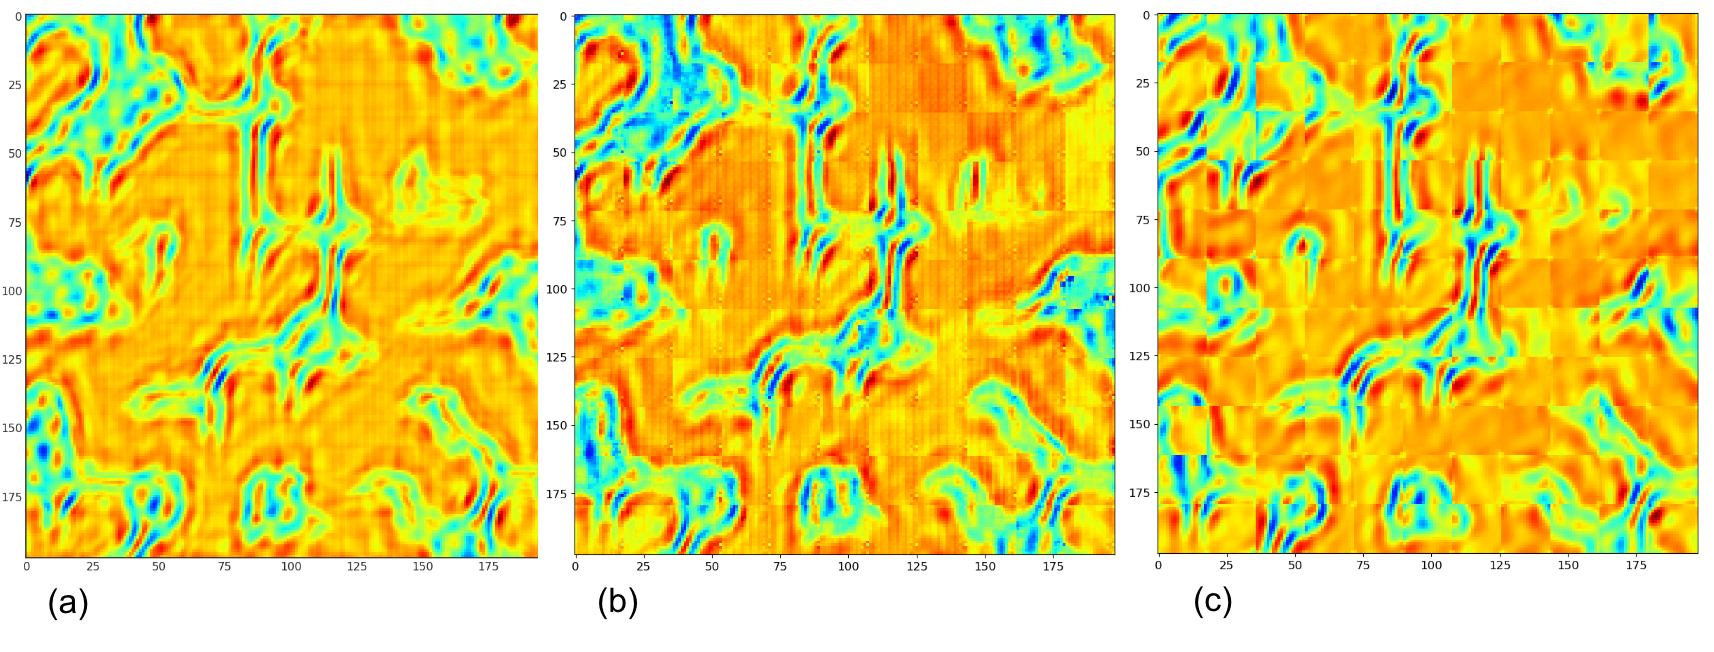
\includegraphics[width=0.9\textwidth]{figures/experimental.png}
%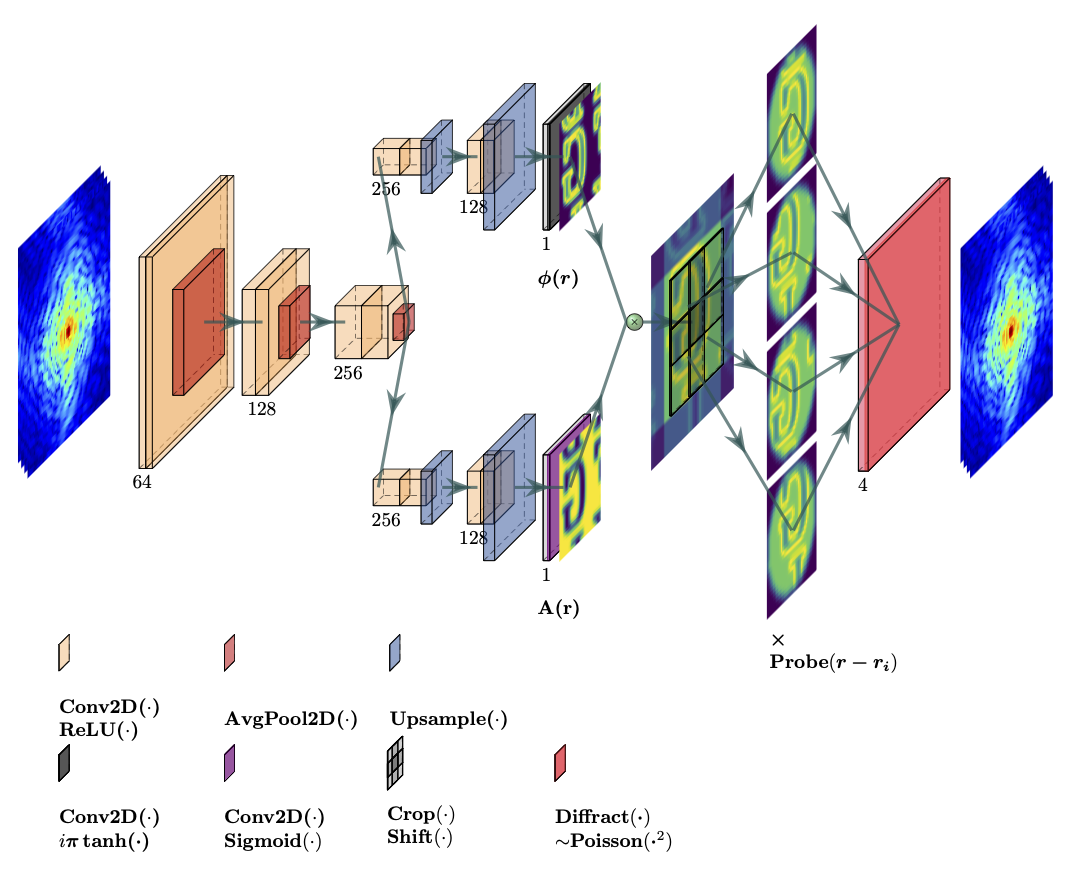
\includegraphics[width=0.9\textwidth]{figures/lett.png}


\begin{figure}[h]%
\centering
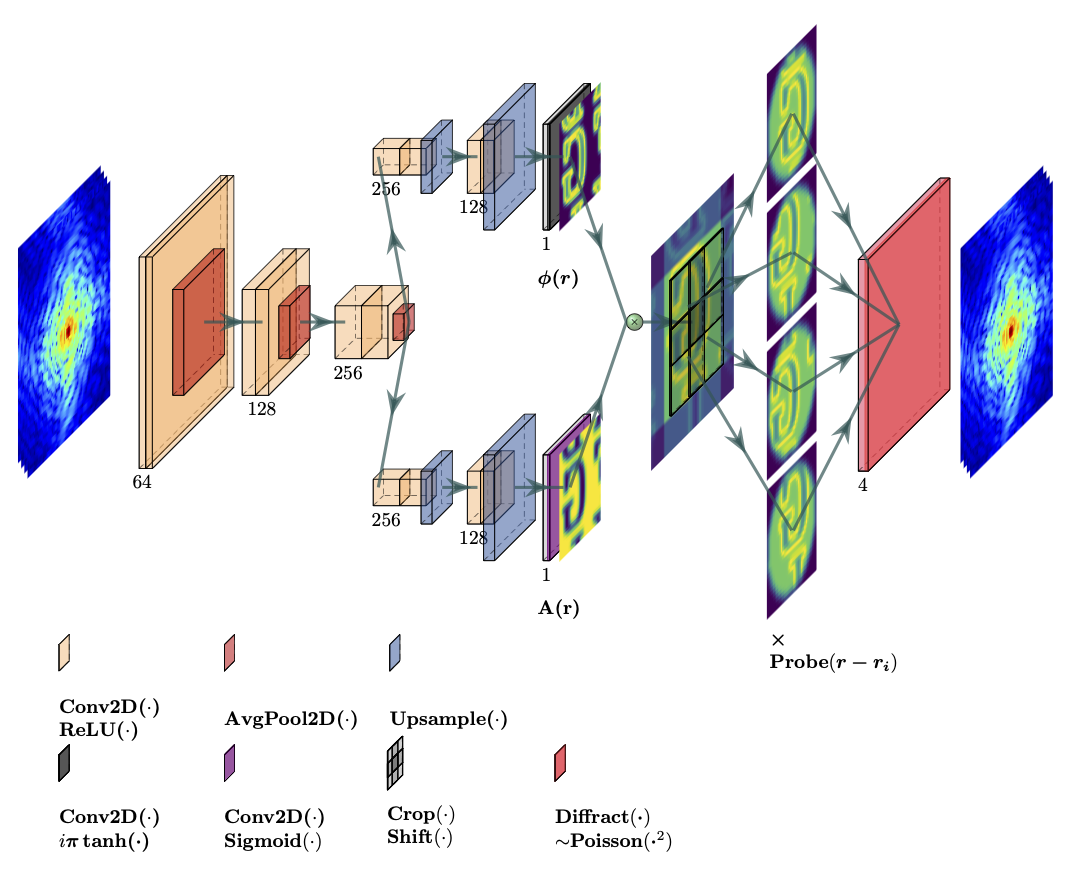
\includegraphics[width=0.9\textwidth]{figures/lett.png}
\caption{Neural network architecture and training configuration of the PtychoPINN model.}\label{diagram}
\end{figure}

\begin{figure}%
    \centering
%    \subfloat[\centering Ground truth]{{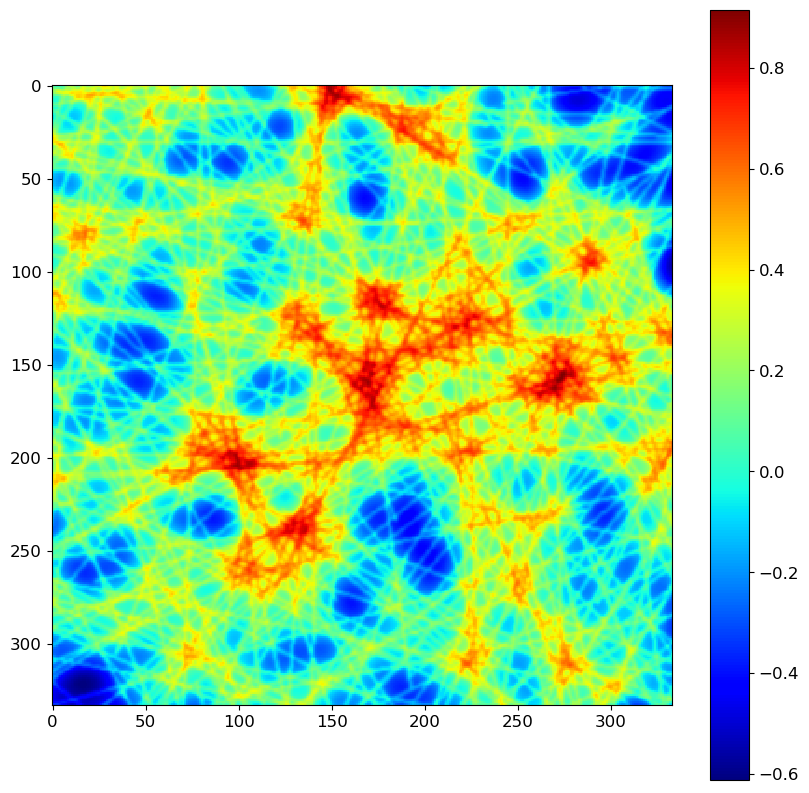
\includegraphics[width=4cm]{figures/gt_phi.png} }}%
%    \subfloat[\centering PtychoNN]{{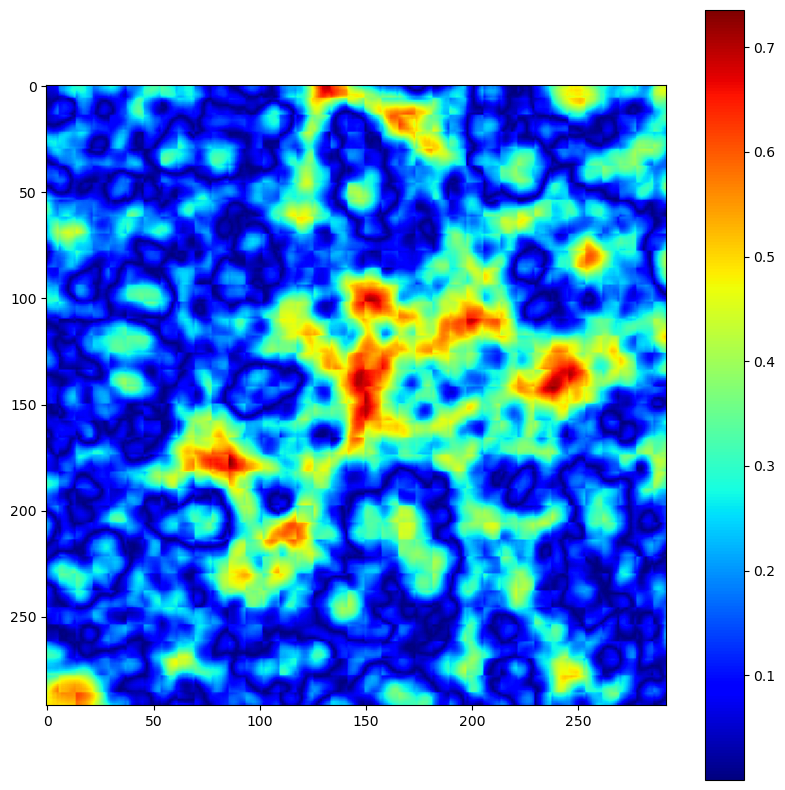
\includegraphics[width=4cm]{figures/PtychoNN_phi.png} }}%
%    \subfloat[\centering PtychoPINN]{{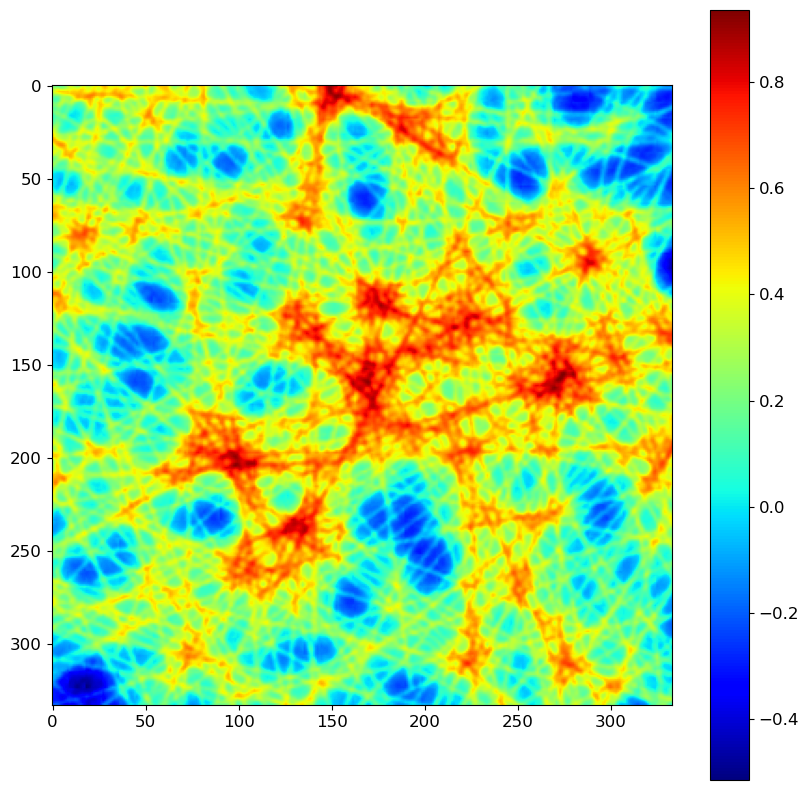
\includegraphics[width=4cm]{figures/PtychoPINN_phi.png} }}%
    \subfloat[\centering Ground truth $\phi$]{{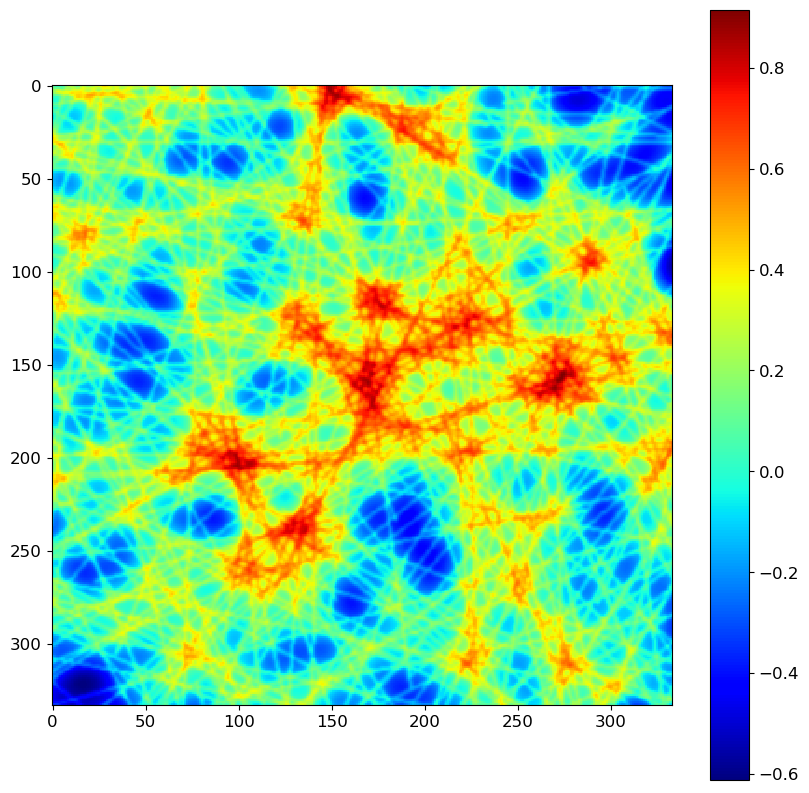
\includegraphics[width=4cm]{figures/gt_phi.png} }}%
    \subfloat[\centering PtychoNN $\phi$]{{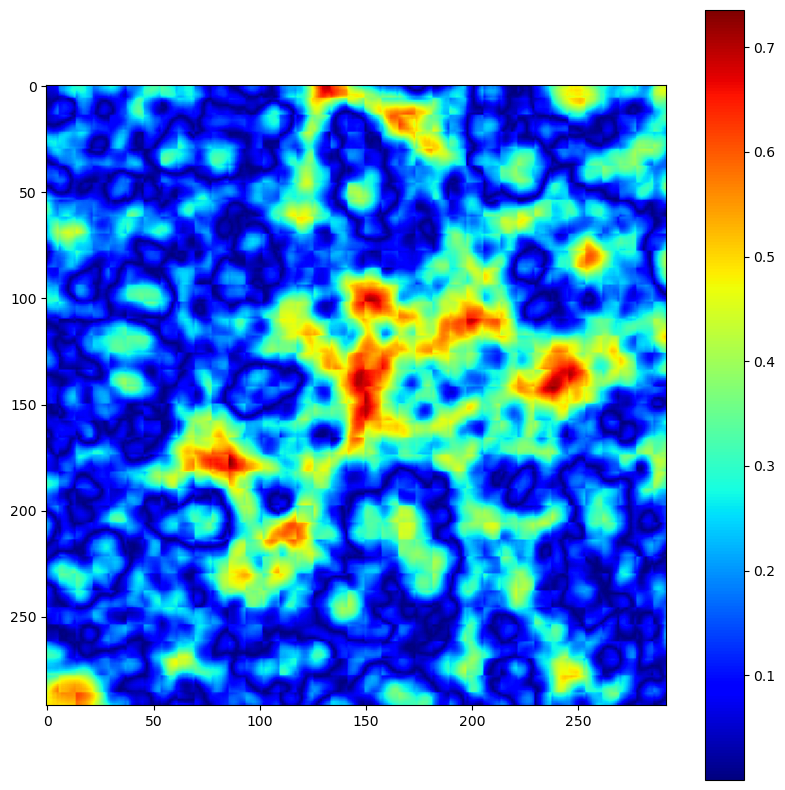
\includegraphics[width=4cm]{figures/PtychoNN_phi.png} }}%
    \subfloat[\centering PtychoPINN $\phi$]{{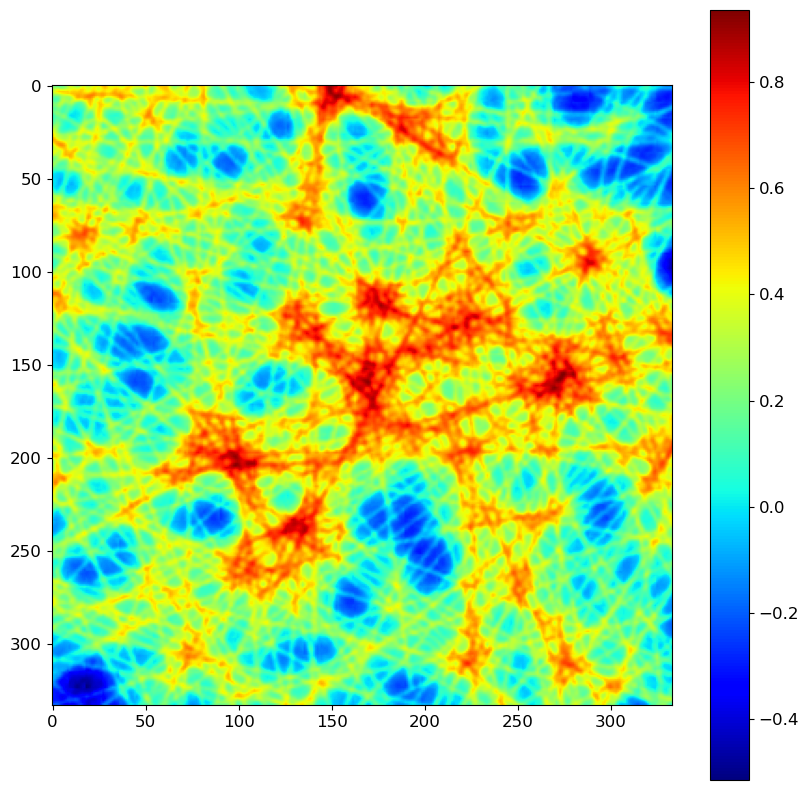
\includegraphics[width=4cm]{figures/PtychoPINN_phi.png} }}%
\vfill
    \subfloat[\centering Ground truth $A$]{{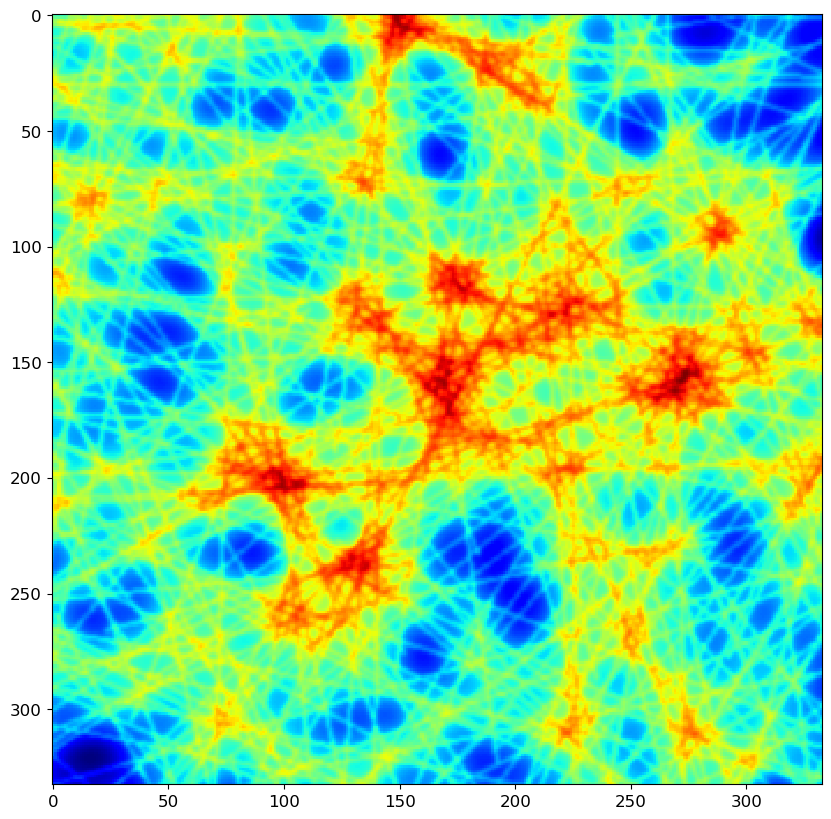
\includegraphics[width=4cm]{figures/ground_truth.png} }}%
    \subfloat[\centering PtychoNN $A$]{{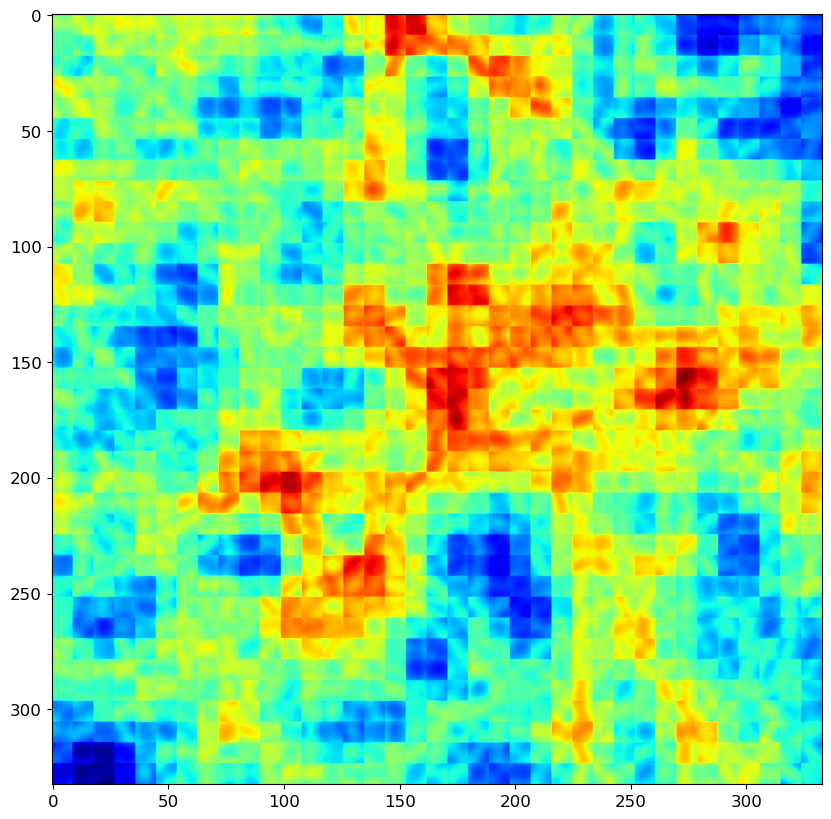
\includegraphics[width=4cm]{figures/ptychoNN.png} }}%
    \subfloat[\centering PtychoPINN $A$]{{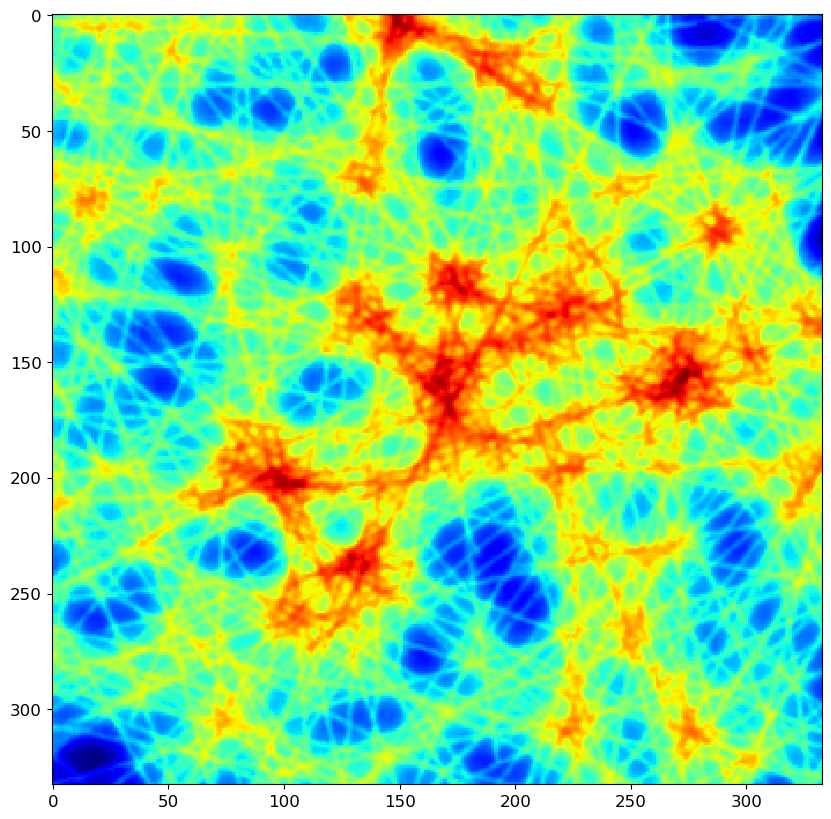
\includegraphics[width=4cm]{figures/PINN.png} }}%
    \caption{Reconstruction comparison, simulated data}%
    \label{fig:sim_comparison}%
\end{figure}

\begin{table}[h]
\begin{center}
\caption{Three reconstruction metrics for the baseline NN reconstruction model and several variations of the PINN architecture, repeated for three contrasting datasets (lines, GRF and experimental). The metrics are mean absolute error (MAE), peak signal to noise (PSNR), and the 50 percent threshold of the Fourier Ring Correlation (FRC50). }\label{tab1}%
\begin{tabular}{p{2cm}l|ll|ll|ll}
\toprule 
    %Model features & \multicolumn{1}{c}{} & \multicolumn{2}{c}{lines} & \multicolumn{2}{c}{GRF} & \multicolumn{2}{c}{experimental}\\
    & \multicolumn{1}{c}{} & \multicolumn{2}{c}{experimental} & \multicolumn{2}{c}{GRF} & \multicolumn{2}{c}{lines}\\
    \midrule
    &
    & $A$ & $\phi$
    & $A$ & $\phi$
    & $A$ & $\phi$ \\
    \midrule
$\{\}$\footnotemark[1]    
& MAE & 0.00394 & 0.542 & 0.0181 & 0.0458 & 0.0245 & 0.13 \\
& PSNR (db) & 92.9  & 50.6 & 80.9 & 71.9 & 40.4 & 62.8 \\
& FRC50 & 34 & 5 & 56 & 53 & 51 & 3 \\
    \midrule
$\mathrm{PINN} $
& MAE & 0.00598 & 0.495 & 0.0371 & 0.11 & 0.0386 & 0.164 \\
& PSNR (db) & 88.8  & 52.4 & 67 & 65.3 & 65 & 63.2 \\
& FRC50 & 8 & 8 & 26 & 6 & 25 & 11.5 \\
    \midrule
overlaps
& MAE & 0.00343 & 0.549 & 0.0166 & 0.0364 & 0.0269 & 0.187 \\
& PSNR (db) & 93.2  & 50.7 & \textbf{81.5} & 74.6 & 41 & 60.3 \\
& FRC50 & \textbf{39} & 1 & 62 & 6 & 49.5 & 2 \\
    \midrule
PINN,overlaps\footnotemark[2]    
& MAE & \textbf{0.00287} & \textbf{0.147} & \textbf{0.00543} & \textbf{0.012} & \textbf{0.00757} & \textbf{0.0208} \\
& PSNR (db) & \textbf{95.8}  & \textbf{61.1} & 80.5 & \textbf{84.5} & \textbf{60.9} & \textbf{79.7} \\
& FRC50 & \textbf{39} & \textbf{51} & \textbf{94} & \textbf{94} & \textbf{170} & \textbf{173} \\
\end{tabular}
\end{center}
\footnotetext[1]{supervised baseline}
\footnotetext[2]{full PtychoPINN}
\end{table}

\begin{figure}%
    \centering
    \subfloat[\centering Ground truth $\phi$]{{\includegraphics[width=4cm]{figures/gt_phi_experimental.png} }}%
    \subfloat[\centering PtychoNN $\phi$]{{\includegraphics[width=4cm]{figures/PtychoNN_phi_experimental.png} }}%
    \subfloat[\centering PtychoPINN $\phi$]{{\includegraphics[width=4cm]{figures/PtychoPINN_phi_experimental.png} }}%
\vfill
    \subfloat[\centering Ground truth $A$]{{\includegraphics[width=4cm]{figures/ground_truth_experimental.png} }}%
    \subfloat[\centering PtychoNN $A$]{{\includegraphics[width=4cm]{figures/ptychoNN_experimental.png} }}%
    \subfloat[\centering PtychoPINN $A$]{{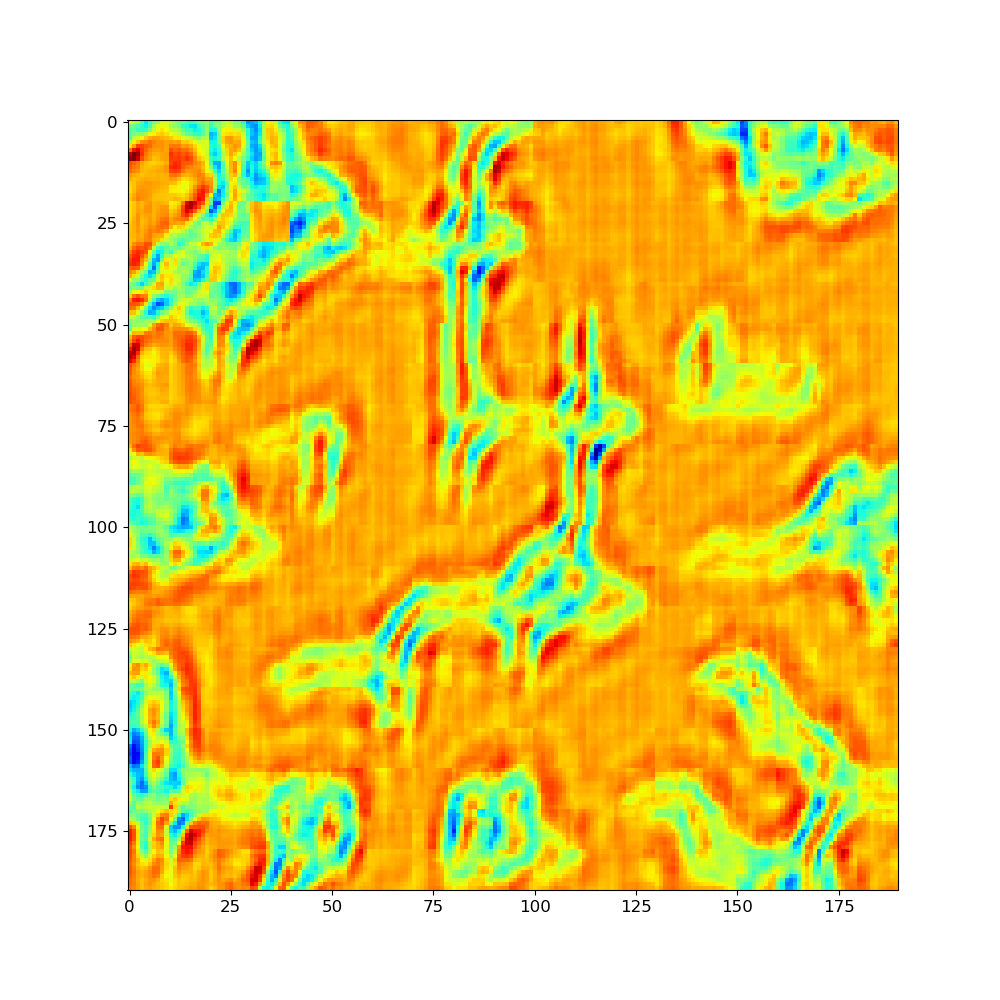
\includegraphics[width=4cm]{figures/PINN_experimental.png} }}%
    \caption{Reconstruction comparison, experimental data}%
    \label{fig:exp_comparison_detailed}%
\end{figure}

\begin{figure}%
    \centering
    \subfloat[\centering GRF dataset]{{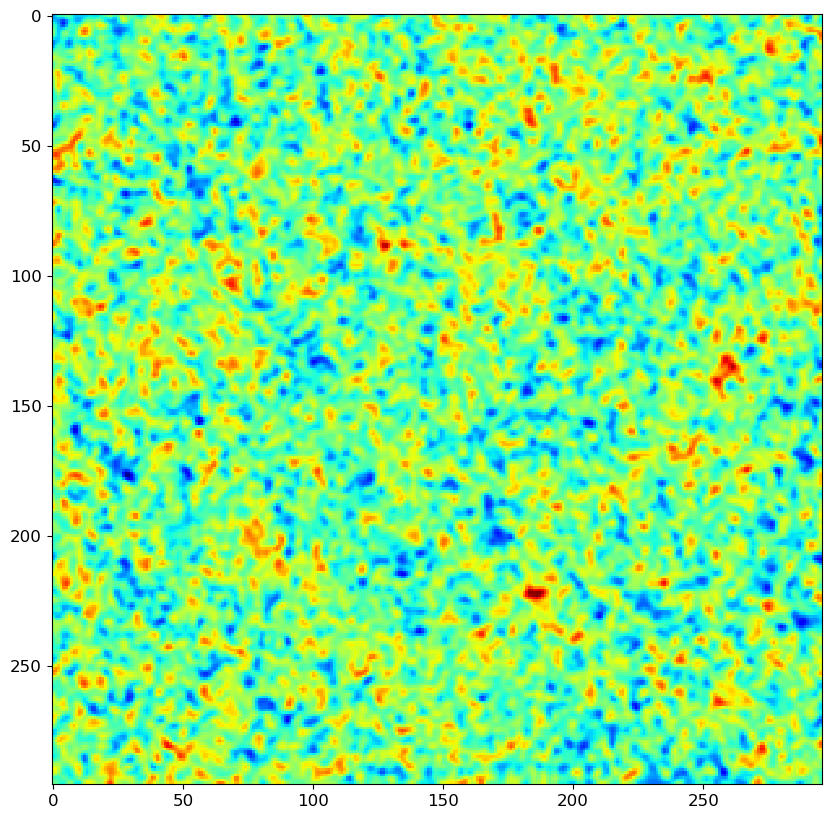
\includegraphics[width=4cm]{figures/GRF.png} }}%
    \caption{Gaussian random field dataset}%
    \label{fig:sim_comparison}%
\end{figure}

\begin{figure}%
    \centering
    \subfloat[\centering Ground truth]{{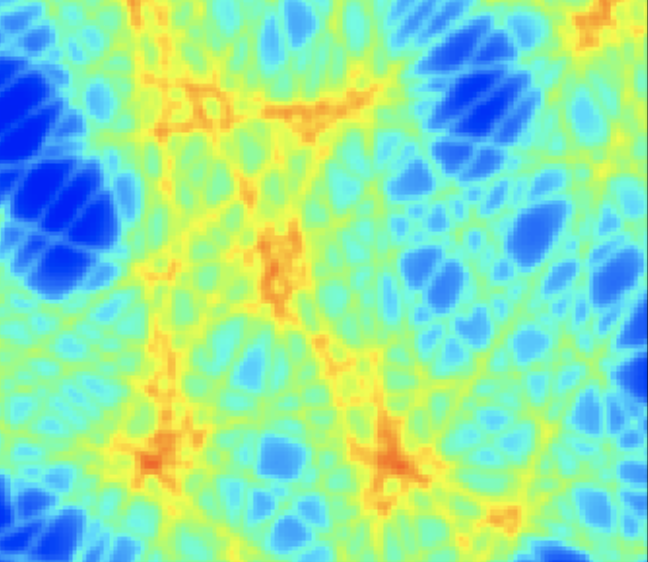
\includegraphics[width=4cm]{figures/generalizability_gt.png} }}%
    \subfloat[\centering PtychoNN]{{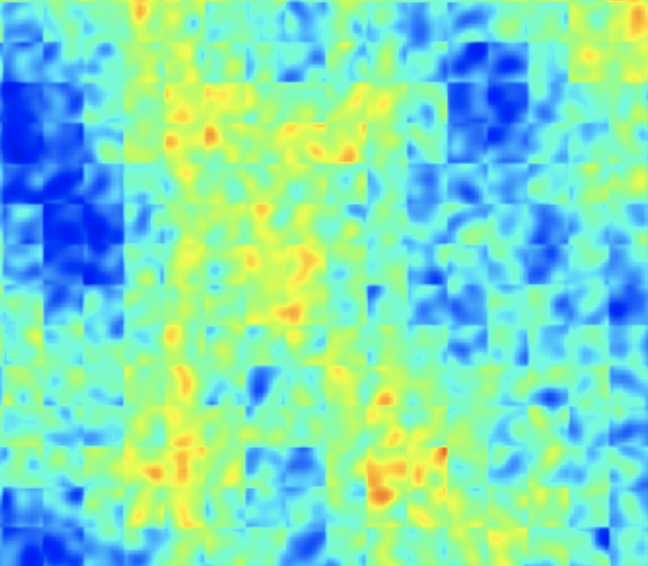
\includegraphics[width=4cm]{figures/generalizability_PtychoNN.png} }}%
    \subfloat[\centering PINN]{{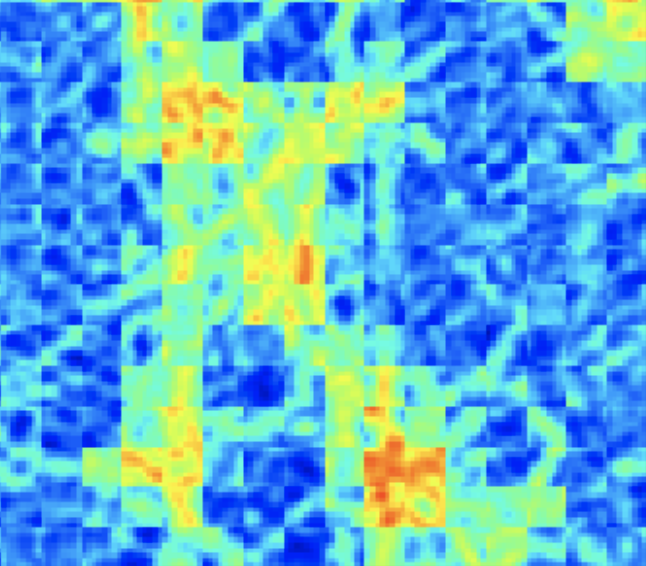
\includegraphics[width=4cm]{figures/generalizability_PINN.png} }}%
    \caption{Test of generalizability}%
    \label{fig:sim_comparison}%
\end{figure}


% \begin{figure}%
%     \centering
%     \subfloat[\centering Ground truth]{{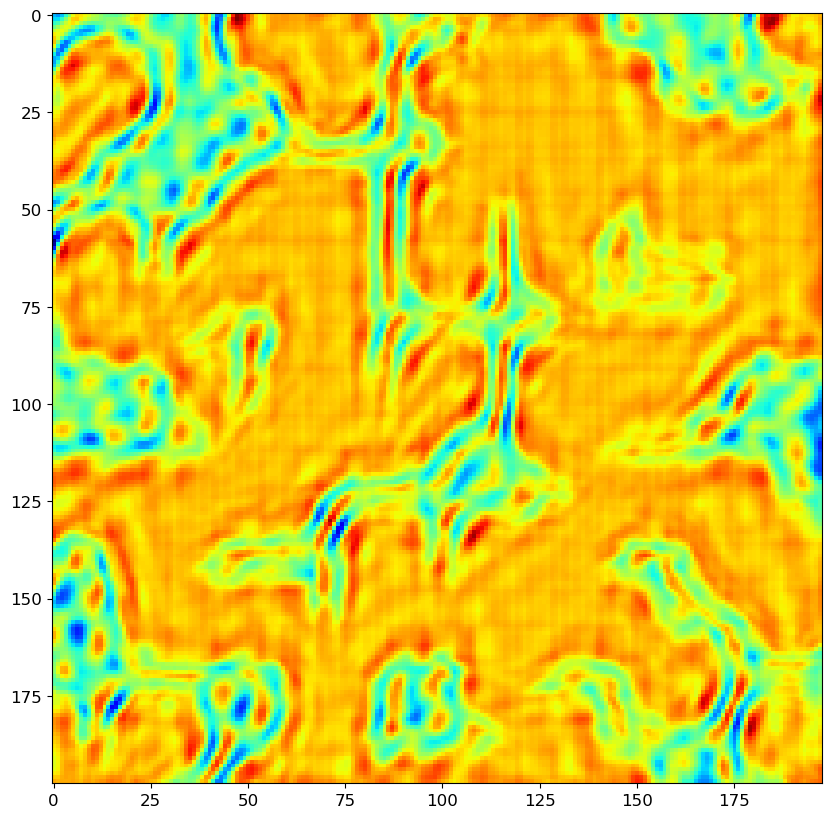
\includegraphics[width=4cm]{figures/gt_experimental.png} }}%
%     \subfloat[\centering PtychoNN]{{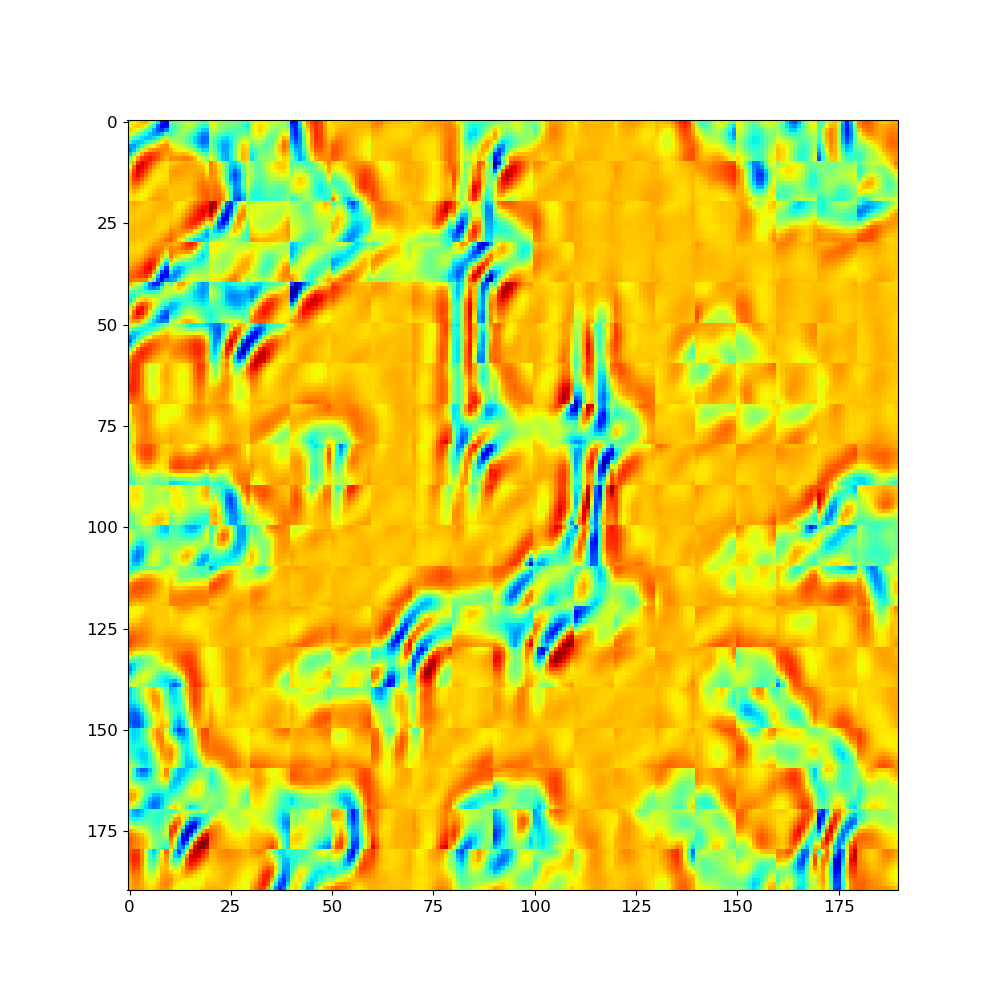
\includegraphics[width=4cm]{figures/PtychoNN_experimental.png} }}%
%     \subfloat[\centering PtychoPINN]{{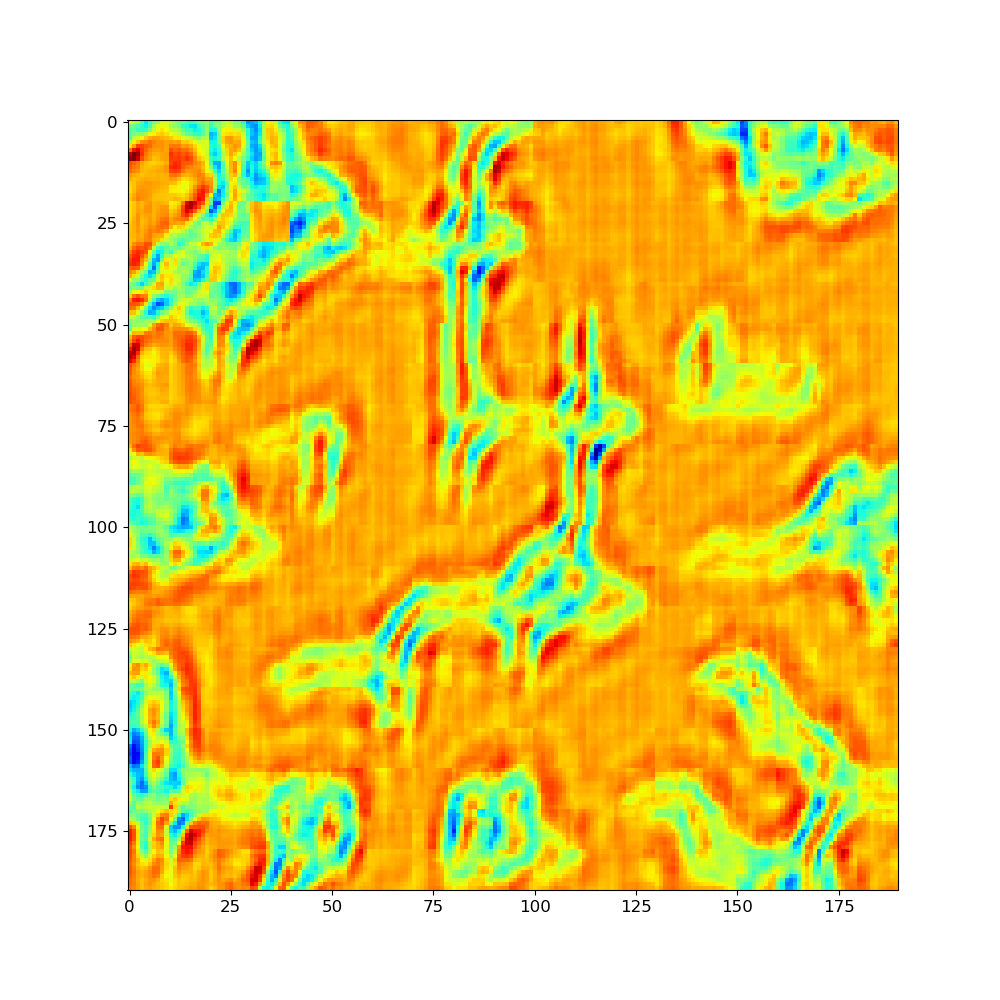
\includegraphics[width=4cm]{figures/PINN_experimental.png} }}%
%     \caption{Reconstruction comparison, experimental data. }%
%     \label{fig:exp_comparison}%
% \end{figure}



%\begin{table}[h]
%\begin{center}
%\caption{Three reconstruction metrics for the baseline NN reconstruction model and several variations of the PINN architecture, repeated for three contrasting datasets (lines, GRF and experimental). The metrics are mean absolute error (MAE), peak signal to noise (PSNR), and the 50 percent threshold of the Fourier ring correlation (FRC50) }\label{tab3}%
%\begin{tabular}{p{2cm}l|ll|ll|ll}
%\toprule 
%    & \multicolumn{1}{c}{} & \multicolumn{2}{c}{experimental} & \multicolumn{2}{c}{GRF} & \multicolumn{2}{c}{lines}\\
%    \midrule
%    &
%    & $A$ & $\phi$
%    & $A$ & $\phi$
%    & $A$ & $\phi$ \\
%    \midrule
%$\{\}$ \footnotemark[1]    
%& MAE & 0.00394 & 0.542 & 0.0181 & 0.0458 & 0.0245 & 0.13 \\
%& PSNR & \textbf{92.5} & 50.6 & 80.9 & 71.9 & 40.4 & 62.8 \\
%& FRC50 & 34 & 5 & 56 & 53 & 51 & 3 \\
%    \midrule
%$\{$overlaps$\}$
%& MAE & \textbf{0.00343} & \textbf{0.549} & \textbf{0.0166} & \textbf{0.0364} & 0.0269 & 0.187 \\
%& PSNR & 93.9 & 50.4 & \textbf{81.5} & \textbf{74.6} & 41 & 60.3 \\
%& FRC50 & 39 & 1 & 62 & 6 & 49.5 & 2 \\
%    \midrule
%$\{\mathrm{PINN}  \}$
%& MAE & 0.00598 & 0.495 & 0.0371 & 0.11 & 0.0386 & 0.164 \\
%& PSNR & 53.8 & 52 & 67 & 65.3 & 65 & 63.2 \\
%& FRC50 & 8 & 8 & 26 & 6 & 25 & 11.5 \\
%    \midrule
%$\{$PINN,~overlaps$\}$
%& MAE & \textbf{0.00287} & 0.147 & 0.00543 & 0.012 & \textbf{0.00757} & \textbf{0.0208} \\
%& PSNR & 54.8 & \textbf{60.8} & 80.5 & \textbf{84.5} & \textbf{60.9} & \textbf{79.7} \\
%& FRC50 & 39 & \textbf{51} & \textbf{94} & \textbf{94} & \textbf{170} & \textbf{173} \\
%    \bottomrule
%\end{tabular}
%\end{center


%In this table, we need 
%a) Additional datasets to test on (can be just one more, but needs to be different). To report the robustness of results.
%b) Do we have the variation about the mean? Was there significant variation due to the ordering of batches, initializations, etc in repeated experiments?
% a) is pretty much required.





\backmatter


\bmhead{Supplementary information}

\section*{Declarations}

\begin{itemize}
\item Funding
\end{itemize}


%%===================================================%%
%% For presentation purpose, we have included        %%
%% \bigskip command. please ignore this.             %%
%%===================================================%%
\bigskip


\begin{appendices}

\section*{Miscellaneous}
\begin{itemize}

\item The underlying manifold on which solutions live is smaller than the 64 x 64 output size ( oversampling requirement). Unsupervised models that are aware of this (e.g. AutophaseNN, PtychoPINN) thus have an output space of the correct (i.e. smaller) size. This may in part explain the PINN's better generalization / performance even in the absence of overlap information. We haven't mentioned this in the text, could go under Discussion / generalization.
\item cite ansel adams print \cite{adams1944mount}
\end{itemize}

% \begin{table}[h]
% \begin{center}
% \caption{Reconstruction accuracy (test MAE) for the baseline NN reconstruction model and several variations of the PINN architecture, repeated for three contrasting datasets. }\label{tab2}%
% \begin{tabular}{p{2cm}llllll}
% \toprule 
%     Model features & \multicolumn{2}{c}{lines} & \multicolumn{2}{c}{GRF} & \multicolumn{2}{c}{experimental}\\
%     & MAE($A$) & MAE($\phi$)
%     & MAE($A$) & MAE($\phi$)
%     & MAE($A$) \\%& MAE($\phi$) \\
%     \midrule
% $\{\}$ \footnotemark[1]    & 0.036   & 0.12  & 0.027 & 0.045 & 0.028 \\
% $\{\mathrm{PINN}  \}$  & 0.036   & 0.077 & 0.049 & 0.088 & 0.039 \\
% $\{$overlaps$\}$  & 0.025 & 0.19 &  0.020 & 0.033 & 0.027 \\
% $\{$PINN,~overlaps$\}$   & 0.0077 & 0.019 & 0.0077 & \bf{0.011} & 0.025 \\
%   $\{$PINN,~NLL$\}$     & 0.043    &   0.18  & 0.049 & 0.12 &  0.038 \\
%   $\{$PINN,~NLL,\newline
%  ~~overlaps$\}$     & \bf{0.0076}    &   \bf{0.014}  & \bf{0.0078} & .012 &  \bf{0.022}  \\
%     \bottomrule
% \end{tabular}
% \end{center}
% \footnotetext[1]{PtychoNN baseline}
% \end{table}

%%=============================================%%
%% For submissions to Nature Portfolio Journals %%
%% please use the heading ``Extended Data''.   %%
%%=============================================%%

%%=============================================================%%
%% Sample for another appendix section			       %%
%%=============================================================%%

%% \section{Example of another appendix section}\label{secA2}%
%% Appendices may be used for helpful, supporting or essential material that would otherwise 
%% clutter, break up or be distracting to the text. Appendices can consist of sections, figures, 
%% tables and equations etc.

\end{appendices}

%%===========================================================================================%%
%% If you are submitting to one of the Nature Portfolio journals, using the eJP submission   %%
%% system, please include the references within the manuscript file itself. You may do this  %%
%% by copying the reference list from your .bbl file, paste it into the main manuscript .tex %%
%% file, and delete the associated \verb+\bibliography+ commands.                            %%
%%===========================================================================================%%

\bibliography{ptycho-pinn}% common bib file
%% if required, the content of .bbl file can be included here once bbl is generated
%%\input sn-article.bbl

%% Default %%
%%\input sn-sample-bib.tex%

\end{document}
